\documentclass[algorithm,
pgfplots,
colortheme=light,
%handout
]{cuzbeamer}

\usepackage[ngerman]{babel}
\usepackage[scale=2]{ccicons}
\usepackage{listings}
\usepackage{csquotes}
\usepackage{xcolor}
\usepackage{hyperref}

\newcommand{\py}[1]{\mintinline{python}{#1}}
\newcommand{\pybw}[1]{\mintinline[style=bw]{python}{#1}}
\newcommand{\bash}[1]{\mintinline{bash}{#1}}
\newcommand{\spacechar}{\texttt{\char32\hspace{2pt}}}

\definecolor{highlightdark}{RGB}{203,236,157}
\definecolor{highlight}{RGB}{79,107,139}





\newcommand{\console}[1]{\texttt{\color{\highlightcolor}#1}}

\let\oldquote\quote
\let\endoldquote\endquote
\renewenvironment{quote}[2][]
{\if\relax\detokenize{#1}\relax
	\def\quoteauthor{#2}%
	\else
	\def\quoteauthor{#2~---~#1}%
	\fi
	\oldquote}
{\par\nobreak\smallskip\hfill(\quoteauthor)%
	\endoldquote\addvspace{\bigskipamount}}



%\newenvironment{mysolution}{\begin{frame}<beamer:0>[fragile]\begin{exampleblock}{Lösung}\begin{minted}{python}}%
%		{\end{minted}\end{exampleblock}\end{frame}}


%\newtheorem{solutionblock}{Example}
\newenvironment<>{solutionblock}[1]{%
\setbeamercolor{block title example}{fg=cyan!60!white}%
\setbeamercolor{itemize item}{fg=cyan!60!white}%
\begin{exampleblock}<beamer:0>{#1}
\vspace{2pt}
	
}%
{\end{exampleblock}}




\begin{document}
\title{Programmieren mit Python}
\author{Dr. Aaron Kunert}
\email{aaron.kunert@salemkolleg.de}
%\subtitle{Teil 11: APIs}
%\date{13. Dezember 2021}

\subtitle{Eine Einführung}
\date{\today}
\maketitle



\section{Zu Beginn \dots}

\begin{frame}
\begin{block}{Kurze Vorstellungsrunde}
	\vspace{2pt}
	Schaffst Du es \emph{in 60 Sekunden} folgende Fragen möglichst knackig und aussagekräftig zu beantworten?
	\begin{itemize}
		\item Wer bist Du? 
		\item Windows, Mac oder Linux?
		\item Welche Vorkenntnisse hast Du beim Programmieren?  
		\item Warum hast Du Dich zum Python-Kurs angemeldet? 
		\item Wann wäre der Kurs für Dich perfekt gelaufen? (Best Case Szenario)
		\item Wann würdest Du den Kurs nicht weiter besuchen? (Worst Case Szenario)
	\end{itemize}
\end{block}
\end{frame}


\begin{frame}
	\begin{block}{Organisation des Kurses}
		\pause 
		\begin{itemize}[<+->]
			\item Ich bin die nächsten 3 Wochen verreist. D.h. nächster Termin am 21. Oktober 
			\item Pausen: Je 20-30 Minuten zum Frühstück und einmal gegen ca. 11 Uhr. Bitte danach pünktlich kommen! 
			\item Skript und alle Unterlagen sind im FirstClass
			\item Gelegentlich gibt es ein Aufgabenblatt (FirstClass) $\rightarrow$ Ca. 5 Tage Bearbeitungszeit, Abgabe per Email $\rightarrow$ individuelles Kurzfeedback
			\item Lernleistung durch: Anwesenheit, Mitarbeit und Bearbeitung der Aufgabenblätter 
			\item Wissenschaftliche Arbeit ist möglich
			\item Kommunikation erstmal per E-Mail
			\item Fragen sind immer und über alle Kanäle willkommen!
		\end{itemize}
	\end{block}
\end{frame}


\begin{frame}
	\begin{block}{Didaktik des Kurses}
		\begin{itemize}
			\item Mischung aus Vortrag, Präsenzübungen und Live-Coding
			\item Lösungen der Präsenzübungen gibt's im Handout im Firstclass
			\item Achtung: Präsenzübungen können erstmal frustrierend sein. 
			\item Im Idealfall: Mehr Praxis statt Erklärungen
		\end{itemize}
	\end{block}
\end{frame}

\begin{frame}
	\begin{block}{Ziele des Kurses}
		\begin{itemize}
			\item Einblick in die \enquote{Denkweise} eines Computers
			\item Einige universelle Konzepte von Programmiersprachen kennenlernen
			\item Schulung des analytischen Denkens
			\item Verständnis von Python-Syntax
			\item Programmierung eines rudimentären Quizspiels
		\end{itemize}
	\end{block}
\end{frame}

\begin{frame}
	\begin{block}{Wo findet man Hilfe/Infos?}
		\vspace{2pt}
		\begin{itemize}
			\item Google
			\item \texttt{stackoverflow.com}
			\item Youtube (z.B. Tutorials)
			\item \texttt{docs.python.org/3}
			\item Bücher (z.B. \textit{Python Crashkurs} v. \textsc{Eric Matthes})
			\item \texttt{mailto: aaron.kunert@salemkolleg.de}
		\end{itemize}
	\end{block}
\end{frame}


\section{Was ist Python?}

\begin{frame}

\begin{block}{Wie funktioniert überhaupt die Programmierung in Python?}
	
	\begin{enumerate}
		\item Man \textbf{schreibt} eine Abfolge von Befehlen/Anweisungen in eine Text-Datei (nicht Word!) 
		\item Danach lässt man diese Datei vom Python-Interpreter \textbf{ausführen}. 
	\end{enumerate}
\end{block}
\end{frame}

\begin{frame}
\metroset{block=fill}
\uncover<+->{\begin{block}{Was wird benötigt?}
		\vspace{2pt}
		\uncover<+->{
			\textbf{Am Anfang}
			\begin{itemize}
				\item Compiler/Interpreter
				\item Texteditor (z.B. Mac: Xcode, Windows: Edit)
			\end{itemize}
		}
		\uncover<+->{
			\textbf{Später}
			\begin{itemize}
				\item Google
				\item Integrierte Entwicklungsumgebung (IDE)
				\item Versionskontrolle (VCS)
				\item Virtueller Maschinen
				\item Datenbanken
				\item Grafikbearbeitung
			\end{itemize}
		}
\end{block}}
\pause 
Editor und Compiler müssen nicht auf dem eigenem Computer installiert sein. Es gibt dafür auch cloudbasierte Lösungen. 
\end{frame}

\begin{frame}
	\begin{block}{Warum Python?}
		\begin{itemize}
			\item Einfaches Setup
			\item Einstiegsfreundliche Syntax
			\item Python ist eine Hochsprache
			\item Python muss nicht kompiliert, sondern nur interpretiert werden
			\item Große Community $\rightarrow$ großes \emph{Ecosystem}
			\item Python ist extrem vielseitig
			\item Python ist plattformunabhängig
		\end{itemize}
	\end{block}
\end{frame}

\begin{frame}
	\begin{block}{Typische Einsatzbereiche}
		\begin{itemize}
			\item Automatisierung
			\item Webscraping
			\item Datenanalyse
			\item Webentwicklung
		\end{itemize}
	\end{block}
\end{frame}





\section{Wie Programmierer denken \\ \footnotesize{Wie lernt man analytisches Denken?}}

\begin{frame}
\begin{quote}{Steve Jobs}
	Everyone in this country should learn to program a computer, because it teaches you to think.
\end{quote}
\end{frame}



\begin{frame}
\begin{block}{Phasen des Lernens einer Programmiersprache}
\vspace{2pt}
\uncover<+->{
	\begin{enumerate}[<+->]
		\item Annäherung:  Fokus auf dem Begreifen der Grundkonzepte
		\item Syntax: Fokus auf der korrekten Anwendung der Syntax
		\item Funktionalität: Fokus liegt darauf, Problemstellungen \emph{pragmatisch} zu lösen
		\item Design: Fokus auf les-und wartbaren Code
		\item Architektur: Fokus auf Strategie, Projekte nachhaltig und erweiterbar umzusetzen 
	\end{enumerate}
}
\end{block}
\end{frame}

\begin{frame}

\begin{block}{Problem Solving}
\vspace{2pt}
Sobald man die Syntax korrekt verwenden kann, steht das Lösen von Problemen beim Programmieren im Fokus.

\pause 

Dabei ist die Kunst nur wenige, klare begrenzte Bausteine (die Befehle der Sprache) \emph{kreativ} so zusammenzusetzen, damit das gegebene Problem gelöst wird. 
\end{block}
\end{frame}

\begin{frame}
\begin{block}{Problemlösungsstrategien}
	\pause 
	\begin{itemize}[<+->]
		\item \textbf{Trial} and Error
		\item Formuliere laut und möglichst präzise, was eigentlich die Problemstellung ist
		\item Zerlege das Problem in kleinere Probleme oder mach Dir Zwischenziele
		\item Gibt es schon eine ähnliches Problem, was Du gelöst hast und von wo aus Du starten kannst?
		\item Erkläre anderen das Problem und was Du schon bisher geschafft hast
		\item Ändere Dein Denken: Scheitern ist nicht das Ende des Weges, sondern der Anfang
		\item To be continued
	\end{itemize}
\end{block}
\end{frame}



\section{Die Konsole \\ \footnotesize{Das Sprachrohr zum Computer}}


\begin{frame}

\metroset{block=fill}
\begin{block}{Definition: Konsole}
	\vspace{2pt}
	Die Konsole ist ein simples Programm, das nur aus einem Eingabefeld besteht, und mit dem man mit einem anderen (in der Regel komplexeren Programm) mittels spezifischer Befehle kommunizieren kann. 
\end{block}

\vspace{10pt}

\pause 

\metroset{block=transparent}

\begin{exampleblock}{Beispiele}
	\begin{itemize}
		\item Windows-Eingabeaufforderung (Kommunikation mit Windows)
		\item Mac-Terminal (Kommunikation mit MacOs)
		\item Browser-Konsole
		\item Die Python-Konsole
	\end{itemize}
\end{exampleblock}

\pause 

	Für Programmiererinnen ist die Konsole der wichtigste Kommunikationsweg zu ihrem Computerprogramm. 
\end{frame}


\begin{frame}{Übung}
\begin{block}{Überprüfe, ob Python bei Dir installiert ist}
	\begin{enumerate}
		\item Google wie man die Konsole bzw. das Terminal zum Betriebssystem öffnet 
		\item Öffne die Konsole
		\item Prüfe, ob Python installiert ist, indem Du einen der folgenden Befehle ausprobierst 
		\begin{itemize}
			\item \bash{python --version}
			\item \bash{python3 --version}
		\end{itemize}
		\item Interpretiere die Antwort
	\end{enumerate}	
\end{block}
\end{frame}




\section{Programmieren in der Cloud \\ \footnotesize{Schnell und unkompliziert einsteigen}}

\begin{frame}
\begin{block}{Browserbasierte IDE verwenden}
	\vspace{2pt}
\begin{enumerate}
\item Gehe auf https://replit.com
\item Erstelle ein Konto (Sign up)
\item Klicke auf \enquote{Create repl}
\item Wähle als Template \enquote{Python} aus
\end{enumerate}
\end{block}
\end{frame}


\section{Erste Schritte im REPL \\ \footnotesize (Read-Evaluate-Print-Loop)}


\begin{frame}
\begin{block}{Probier mal folgende Kommandos aus}	
	\begin{itemize}
		\item \py{3 + 4}
		\item \py{2 - 7}
		\item \py{"Hello" + "World"}
	\end{itemize}
\end{block}	
\end{frame}



\begin{frame}{Übung}
\uncover<+->{\begin{block}{Was machen die folgenden \textit{Operatoren}?}
	\begin{itemize}
		\item \pybw{+}
		\item \pybw{-}
		\item \pybw{*}
		\item \pybw{/}
		\item \pybw{**}
	\end{itemize}
\end{block}}
\uncover<+->{\begin{block}{Und diese?}
\begin{itemize}
		\item \%
		\item \pybw{//}
		\item \pybw{==}
		\item \pybw{<=}
		\item \pybw{<}
\end{itemize}
\end{block}}
\end{frame}

\begin{frame}<beamer:0>[fragile]
\frametitle{Lösungen}
\begin{solutionblock}{Operatoren I}
Die Operatoren 	\pybw{+} und \pybw{-} sind klar. Die Operatoren \pybw{*} und \pybw{/} bezeichnen Multiplikation und Division. 
Der Operator \pybw{**} berechnet die Potenz (hochnehmen). 
\end{solutionblock}

\vspace{12pt}

\begin{solutionblock}{Operatoren II}
	Der Operator \% ist der Modulo-Operator (vgl.  \href{https://de.wikipedia.org/wiki/Division_mit_Rest#Modulo}{Wikipedia}). Der Operator \pybw{//} arbeitet analog zur Divison, rundet das Ergebnis jedoch auf die nächste ganze Zahl ab. Die Operatoren \pybw{==} (Gleichheit), \pybw{<=} (Kleinergleich), \pybw{<} (kleiner als) sind Vergleichsoperatoren und geben entweder \pybw{True} oder \pybw{False} zurück
\end{solutionblock}


\end{frame}




\begin{frame}{Übung}
	\begin{block}{Wie rechnet Python?}
		\begin{itemize}
			\item Wird Punkt-vor-Strich berücksichtigt?
			\item Kann man mit Klammern die Reihenfolge beeinflussen?
			\item Was ist der Unterschied zwischen \py{10/5} und \py{10//5} ?
			\item Was bedeutet das Kommando \py{_}? 
			\item Wie kann man Zwischenergebnisse in Variablen speichern?
		\end{itemize}
	\end{block}
\end{frame}

\begin{frame}<beamer:0>[fragile]
\frametitle{Lösung}
\begin{solutionblock}{Rechenregeln}
	\begin{itemize}
		\item Python rechnet Punkt-vor-Strich.
		\item Python berücksichtigt Klammern.
		\item Das Ergebnis von \py{/} ist stets eine Fließkommazahl, das Ergebnis von \py{//} ist stets eine ganze Zahl. 
		\item Das Kommando \py{_}, referenziert das vorherige Ergebnis. 
		\item Zwischenergebnise lassen sich mittels des Zuweisungsoperators \py{=} in einer Variable speichern. 
	\end{itemize}
\end{solutionblock}
\end{frame}

\section{Variablen}

\begin{frame}
\uncover<+->{\begin{block}{}
		Jeder Wert in Python kann in einer Variable gespeichert werden: 
		
		\py{my_variable = 3}
\end{block}}

\uncover<+->{\begin{block}{}
		Die Zuweisung darf auch das Ergebnis einer Berechnung sein: 
		
		\py{my_new_variable = 3 + 5}
\end{block}}
\uncover<+->{\begin{block}{}
		Die Zuweisung darf auch weitere Variablen enthalten: 
		
		\py{my_brand_new_variable = my_variable + my_new_variable }
\end{block}}

\uncover<+->{\begin{block}{}
	Man darf auch Kettenzuweisungen machen: 
	
	\py{a = b = c = 100 }
\end{block}}
\end{frame}


\begin{frame}
\uncover<+->{\begin{block}{Gültige Variablennamen}
\begin{itemize}[<+->]
	\item Erlaubt sind Buchstaben (nur ASCII), Ziffern und Unterstriche
	\item Der Name darf nicht mit einer Ziffer starten
	\item Beliebige Länge 
	\item Wer's schon kennt als \emph{regulärer Ausdruck}:  \mintinline{php}{[_a-zA-Z][_0-9a-zA-Z]*}
	\item Schlüsselwörter sind nicht erlaubt
\end{itemize} 
\end{block}}
\vspace{12pt}
\uncover<+->{\begin{block}{Liste der Schlüsselwörter}
	\texttt{
	\begin{columns}[T,onlytextwidth]
		\column{0.2\textwidth}
		False\\ 	await\\ 	else\\ 	import\\ 	pass\\ assert \\	del\\ 	
		\column{0.2\textwidth}
		None \\	break \\	except \\ 	in \\	raise \\ global \\	not \\	 
		\column{0.2\textwidth}
		True \\	class \\ 	finally \\ 	is \\	return \\ with \\ async 
		\column{0.2\textwidth}
		and \\	continue \\ 	for \\	lambda \\	try \\ 	elif  \\	if  \\
		\column{0.2\textwidth}
		as \\ 	def \\ 	from  \\	nonlocal \\	while \\ 	or \\ 	yield
	\end{columns}
}
\end{block}}
\end{frame}


\begin{frame}
\uncover<+->{\begin{exampleblock}{Style-Guide Variablennamen}
	\begin{itemize}
		\item Englische Wörter
		\item Nur Kleinbuchstaben
		\item Möglichst aussdrucksstarke Namen verwenden
		\item Keine Angst vor langen Namen 
		\item Namen, die aus mehreren Worten bestehen, mit Unterstrich trennen (\textit{snake-case})
	\end{itemize}
	
	\uncover<+->{z.B. \py{students_in_this_room}, \py{number_of_unpaid_bills}}
\end{exampleblock}}

\end{frame}

\begin{frame}{Übung}
	
	\begin{block}{Probier's aus!}
		\begin{itemize}
			\item Welchen Wert hat eine Variable, wenn man sie nicht vorher definiert hat? 
			\item Was passiert, wenn man eine Variable definiert, die schonmal verwendet wurde?
			\item Wie kann man eine Variable mit Wert \py{3} um \py{1} vergrößern?
		\end{itemize}	
	\end{block}
\vspace{12pt}
\begin{solutionblock}{Lösung}
	\begin{itemize}
		\item Verwendet man eine undefinierte Variable, wird ein Fehler geworfen
		\item Ja, man kann eine Variable einfach neu definieren
		\item Hat beispielsweise \pybw{my_variable} den Wert 3, so lässt sich der Wert wie folgt vergrößern: 
		\pybw{my_variable = my_variable + 1} 
	\end{itemize}
\end{solutionblock}
\end{frame}
	

\section{Datentypen}

\begin{frame}
	\begin{block}{}
		Jeder Wert in Python hat einen \textit{Datentyp}. Unter anderem gibt es folgende \textit{primitive} Typen in Python.
		\begin{itemize}
			\item \py{int}  Integer (ganze Zahlen)
			\item \py{float} Float (Dezimalzahlen)
			\item \py{bool} Boolean (Wahrheitswerte)
			\item \py{str}  String (Zeichenketten)
			\item \pybw{NoneType} (Typ des leeren Werts \py{None})
		\end{itemize}
	\end{block}
\end{frame}


\begin{frame}
	\metroset{block=fill}
	
	\uncover<+->{\begin{block}{Integer}
		Ganze Zahlen wie z.B. \py{1}, \py{-1}, \py{0}. Nicht aber 
		\py{2.0} oder \py{0.0}. 	
	\end{block}}
	\vspace{12pt}
	\uncover<+->{\begin{block}{Float}
		Fließkommazahlen, z.B. \py{3.1415925}. Achtung: Bei Float-Berechnungen können schnell \enquote{Überraschungen} auftreten: Was ergibt z.B. \mintinline{python}{1.2 - 1.0} ? 
	\end{block}}
	\vspace{12pt}
	\uncover<+->{\begin{block}{Boolean}
		Booleans sind eine Sonderform von \py{int} und können nur die Werte \py{True} (entspricht 1) und \py{False} (entspricht 0) annehmen. Sie entstehen in der Regel, wenn man Fragen im Programm stellt (z.B. \py{3 < 4} oder \py{1 == 2}).   	
	\end{block}}
\end{frame}



\begin{frame}
	\metroset{block=fill}
	\uncover<+->{\begin{block}{String}
		Strings sind beliebige Zeichenketten und müssen in (ein-, zwei- oder dreifache) Anführungszeichen eingeschlossen werden. Die Ausdrücke \pybw{'hello'}, \pybw{"Hello"} und \pybw{"""Hello"""} sind (fast) äquivalent. 
	\end{block}}
	\vspace{12pt}
	\metroset{block=transparent}
	\uncover<+->{\begin{block}{Mehrzeilige Strings}
			\vspace{2pt}
		Ein \textit{Stringliteral} kann nur innerhalb einer Zeile definiert werden. Soll ein String mehrere Zeilen umfassen, müssen dreifache Anführungszeichen verwendet werden.  
	\end{block}}

	\end{frame}

	\begin{frame}
		\uncover<+->{\begin{block}{Steuerzeichen}
				\vspace{2pt}
			Gewisse Kombinationen mit Backslash sind reservierte Steuerzeichen. So bezeichnet beispielsweise \py{\n} einen Zeilenumbruch und \py{\t} ein Tabulatorzeichen. \\
			Beispiel: \py{"This text\nfills two lines"}
		\end{block}}
			\vspace{12pt}
		\uncover<+->{\begin{block}{Escaping}
			\vspace{2pt}
			Möchte man ein Steuerzeichen nicht ausführen, sondern buchstäblich nehmen. Muss man sie mit einem Backslash \textit{escapen} bzw. maskieren. \\
			Beispiel: \py{"This text fits in\\n one line"}
		\end{block}}
		\vspace{12pt}
		\uncover<+->{\begin{block}{Raw-Strings}
				\vspace{2pt}
				Möchte man alle Steuerzeichen eines Strings ignorieren, kann man ihn als \textit{Raw-String} definieren. \\
				Beispiel: \py{r"This \n String \t has no control characters"}
		\end{block}}
		
	\end{frame}

	
	\begin{frame}
		\metroset{block=fill}
		\uncover<+->{\begin{block}{Typecasting (Umwandlung von Typen)}
			\vspace{2pt}
			\uncover<+->{\textbf{Implizit}\\
			Bei manchen Operationen nimmt Python automatisch eine Typumwandlung vor. \\ Beispiel: \py{1 + 2.0} ergibt \py{3.0}	
		} \\ \\
		\uncover<+->{\textbf{Explizit \\}
			Die Funktionen \py{int()}, \py{float()}, \py{str()} und \py{bool()} führen jeweils eine Typumwandlung durch (sofern möglich). Beispiele: 
			\begin{itemize}
				\item \py{int(2.0)} ergibt \py{2} 
				\item \py{float(2)} ergibt \py{2.0} 
				\item \py{int("3")} ergibt \py{3}
			\end{itemize} 
		}
		\end{block}}
		
		\vspace{12pt}
		\metroset{block=transparent}
		\uncover<+->{\begin{block}{Typ einer Variablen ermitteln}
			\vspace{2pt}
			Mit der Funktion \py{type()} lässt sich der Typ bestimmen, z.B. \py{type(3.2)}.  	
		\end{block}}
		
	\end{frame}
	
	
	\begin{frame}{Übung}
		\begin{block}{Versuche die Fragen erst ohne Python zu beantworten, überprüfe Deine Vermutung}
			\begin{itemize}
				\item Welchen Datentyp hat das Ergebnis von \py{3 - 1.0} ?
				\item Was ist das Ergebnis von \py{"2" + 1} ? 
				\item Was ist das Ergebnis von \py{"2"} + \py{"2"}? 
				\item Sind die beiden Werte \py{0} und \py{"0"} gleich? 
				\item Sind die beiden Werte \py{2} und \py{True} gleich? 
				\item Sind die beiden Werte \py{bool(2)} und \py{True} gleich? 
				\item Sind die beiden Werte \py{1} und \py{True} gleich? 
			\end{itemize}
		\end{block}
	\end{frame}


\begin{frame}<beamer:0>[fragile]
\frametitle{Lösungen}
\begin{solutionblock}{Typaufgaben}
	\begin{itemize}
		\item Der Datentyp des Ergebnisses ist \pybw{float}
		\item Fehlermeldung
		\item Das Ergebnis ist \py{"22"}
		\item Nein
		\item Nein 
		\item Ja
		\item Ja
	\end{itemize}
\end{solutionblock}
\end{frame}

	\begin{frame}{Übung}
	
	\begin{block}{Erkläre mit Deinen eigenen Worten}
		\begin{itemize}
			\item Nach welcher Regel wandelt \py{int()} eine Fließkommazahl in eine ganze Zahl um? 
			\item Nach welchen Regeln wandelt \py{bool()} Zahlen und Strings in einen Wahrheitswert um? 
		\end{itemize}
	\end{block}
	
	
\end{frame}









\section{Operatoren}

\begin{frame}
\begin{block}{Die wichtigsten Operatoren}
	\begin{itemize}
		\item \pybw{+} (Addition oder Zusammenkleben von Strings)
		\item \pybw{-} (Subtraktion)
		\item \pybw{*} (Multiplikation)
		\item \pybw{/} (Division, ergibt immer ein Wert vom Typ \pybw{float})
		\item \pybw{**} (Potenzierung)
		\item \% (\textit{modulo-Operator}: Rest bei ganzzahliger Division)
		\item \pybw{//} (Division und Abrunden, ergibt immer ein Wert vom Typ \pybw{int})
		\item \pybw{==} (Vergleichsoperator, ergibt immer ein Wert vom Typ \pybw{bool})
		\item \pybw{!=} (Ungleichheitsoperator, ergibt das Gegenteil von \pybw{==})
	\end{itemize}
\end{block}
\end{frame}

\begin{frame}
\begin{block}{Operator-Präzedenz}
\uncover<+->{
	\begin{enumerate}[<+->]
		\item Klammern
		\item \pybw{**}
		\item \pybw{*}, \pybw{/}, \pybw{//}, \%
		\item \pybw{+},\pybw{-}
	\end{enumerate}	
}
\uncover<+->{
	Operatoren gleichen Rangs werden innerhalb eines Ausdrucks von links nach rechts abgearbeitet. 
}

\uncover<+->{
	\vspace{10pt}
	\textbf{Ausnahmen:}\\
	Potenzierung (\py{**}) und Zuweisung (\py{=}) werden von rechts nach links verarbeitet. 
}
\end{block}
\end{frame}

\begin{fragile}[]
\begin{block}{Kombinierte Zuweisung}
\vspace{2pt}
Oft möchte man eine gegebene Variable neu zuweisen: 
\begin{minted}{python}
counter = 1
counter = counter + 1 	# counter = 2
\end{minted}
\pause
Dies lässt sich auch kurz schreiben als 
\begin{minted}{python}
counter = 1
counter += 1 	# counter = 2
\end{minted}
\pause
Analog sind die Operatoren \py{-=}, \py{*=}, \py{/=}, etc. definiert. 
\end{block}
\end{fragile}

\section{Von der REPL zum Quellcode}
\begin{frame}
\begin{block}{Script Mode}
	\vspace{2pt}
	Sobald man mehrere zusammenhängende Zeilen hat, wird die Eingabekonsole (REPL) sehr unübersichtlich. Daher gibt es auch die Möglichkeit, alle Programmzeilen zunächst aufzuschreiben und diese dann gebündelt von Python ausführen zu lassen. Im Gegensatz zum REPL bzw. interactive Mode von Python wird dies \emph{Script Mode} genannt.    
\end{block}
\end{frame}

\begin{fragile}[]
\begin{exampleblock}{Beispiel}
\begin{minted}{python}
name = "Max"
age = 20
age = age + 1
\end{minted}
\end{exampleblock}

\vspace{12pt}

\pause
\begin{block}{Ausführung}
\vspace{2pt}
Um diesen Code auszuführen, muss man bei Replit auf den Run-Button klicken oder alternativ den Shortcut Strg+Enter (Windows) bzw. Cmd+Enter (Mac) verwenden.  
\end{block}

\vspace{12pt}

\pause

\begin{alertblock}{Achtung}
\vspace{2pt}
Im Gegensatz zum REPL werden Ergebnisse von Rechnungen nicht mehr automatisch auf der Konsole ausgegeben. 
\end{alertblock}

\end{fragile}



\section{Input/Output \\ \footnotesize Kommunikation über die Konsole}


\begin{frame}

\begin{block}{Die Konsole}
\vspace{2pt}
Grafische Benutzeroberflächen sind zu Beginn relativ kompliziert, daher verwenden wir zunächst die \emph{Python-Konsole} für die Kommunikation mit unserem Programm. 
\end{block}

\end{frame}

\begin{fragile}[]
	
	\begin{block}{Output}
		\vspace{2pt}
		Um einen String auf der \emph{Konsole} auszugeben, verwende die Funktion \py{print()}. 
		
		
		Zum Beispiel: \py{print("Hello there")}. 
		\pause
		
		\vspace{12pt}
		
		Es können auch Variablen eingesetzt werden: 
		\begin{minted}{python}
		message = "Hello there"
		print(message) # Hello there
		\end{minted}
		
	\end{block}
	
\end{fragile}

\begin{fragile}[]
	
	\begin{block}{String Interpolation}
		\vspace{2pt}
		Um Variablenwerte innerhalb eines Strings auszugeben, verwenden wir die String-Interpolation-Syntax:
		\begin{minted}{python}
		my_value = 5
		print(f"The variable my_value has the value {my_value}")
		# The variable my_value has the value 5
		\end{minted}
		
		\pause
		
		\vspace{12pt}
		
		Das geht auch als \textit{inline expression}: 
		\begin{minted}{python}
		print(f"The sum of 1 and 2 is {1+2}")
		# The sum of 1 and 2 is 3
		\end{minted}
		
	\end{block}
	
\end{fragile}

\begin{fragile}
	\begin{block}{Input}
		\vspace{2pt}
		Um einen String vom User einzulesen, verwende die Funktion \py{input()}:
		
		\begin{minted}{python}
		age = input("How old are you?")
		print(f"I am {age} years old")
		\end{minted}
	\end{block}
	\pause 
	\begin{alertblock}{Achtung}
		\vspace{2pt}
		Das Ergebnis von \py{input} hat stets den Datentyp \py{string} auch wenn Zahlen eingelesen werden. Gegebenenfalls muss das Ergebnis mittels \py{int()} oder \py{float()} in den gewünschten Typ umgewandelt werden. 	
	\end{alertblock}
	
\end{fragile}


\begin{fragile}[]
	\begin{exampleblock}{Beispiel: Input und Output kombiniert}
		\begin{minted}{python}
		name = input("What is your name?")
		age = input("What is your age?")
		print(f"Hello {name}, you are {age} years old") 
		\end{minted}
	\end{exampleblock}
\end{fragile}

\begin{frame}{Übung}
\begin{block}{Adressabfrage}
\vspace{2pt}
Schreibe ein kurzes Skript, dass Dich nach Deinem Namen, Alter und Adresse fragt. Wenn es alles eingelesen hat, soll es diese Infos in folgender Form auf der Konsole ausgeben: 	

\console{Hallo Max, schön dass Du da bist. Du bist 21 Jahre alt und wohnst in der Bismarckstraße 12 in Glücksstadt.}
\end{block}
\end{frame}

\begin{frame}<beamer:0>[fragile]
\frametitle{Lösung}
\begin{solutionblock}{Adressabfrage}
\begin{minted}{python}
name = input("Dein Name: ")
age = input("Dein Alter: ")
street = input("Deine Addresse: ")
city = input("Deine Stadt: ") 

print(f"Hallo {Name}, schön, dass Du da bist. Du bist {age} Jahre alt")
print(f"und wohnst in der {street} in {city}.")
\end{minted}
\end{solutionblock}
\end{frame}



\begin{fragile}[Übung]
\begin{block}{Blick in die Zukunft}
	\vspace{2pt}
Schreibe ein kurzes Skript, dass Dich nach Deinem Alter fragt. Daraufhin soll es auf der Konsole ausgeben, wie alt Du in 15 Jahren sein wirst. 
\end{block}
\vspace{12pt}
\begin{solutionblock}<beamer:0>{Lösung}
\begin{minted}{python}
age = input("Wie alt bist Du? ")
age = int(age) + 15
print(f"In 15 Jahren wirst Du {age} sein.")
\end{minted}
\end{solutionblock}
\end{fragile}

\section{Kommentare}

\begin{fragile}


\begin{block}{Kommentare}
\vspace{2pt}
Alle Zeichen einer Zeile, die hinter einem \texttt{\#} (Hashtag) kommen, werden von Python ignoriert.
So lassen sich Kommentare im Quellcode platzieren. 
\end{block}

\vspace{12pt}

\pause
\begin{exampleblock}{Beispiel}
\begin{minted}{python}
print("This line will be printed")
# print("This line won't") 
\end{minted}
\end{exampleblock}

\end{fragile}



\section{Conditionals \\ \footnotesize Ein Programm verzweigen}

\begin{frame}
	\begin{block}{Problemstellung}
		\vspace{2pt}
		Lies eine Zahl \py{x} ein. In Abhängigkeit von \py{x} soll Folgendes ausgegeben werden: 
		
		\console{Die Zahl x ist größer als 0} 
		
		bzw. 
		
		\console{Die Zahl x ist kleiner 0}  
		\vspace{8pt}
		
		
		Wie macht man das?
		\end{block}
\end{frame}

\begin{fragile}
	
\begin{block}{Lösung \footnotesize(fast)}
\begin{minted}{python}
x = input("Gib eine Zahl x an")
x = int(x)

if x > 0:
  print("x ist größer 0")
else:
  print("x ist kleiner 0")
\end{minted}
\end{block}
	
\end{fragile}


\begin{frame}
\metroset{block=fill}


	\renewcommand{\baselinestretch}{1.5}
\begin{block}{Struktur \texttt{if-else} Statement}	
	\vspace{2pt}
	\uncover<+->{
	\uncover<+->{\texttt{if}} \uncover<+->{\textit{Bedingung}}\uncover<+->{\texttt{:}}\\
	\uncover<+->{\spacechar\spacechar }\uncover<+->{\textit{Codezeile A1}}	\\
	\uncover<+->{\spacechar\spacechar \textit{Codezeile A2}	\\
	\spacechar\spacechar \phantom{Code}\vdots}\\
	\uncover<+->{\texttt{else:}}\\
	\uncover<+->{\spacechar\spacechar \textit{Codezeile B1}	\\
				 \spacechar\spacechar \textit{Codezeile B2}	\\
				 \spacechar\spacechar \phantom{Code}\vdots}\\
	\uncover<+->{\textit{Codezeile C1}\\
	\phantom{Code}\vdots
}
}
\end{block}
\renewcommand{\baselinestretch}{1}
%\vspace{10pt}

\end{frame}
\begin{frame}
\begin{block}{Wie funktioniert's?}
	\vspace{2pt}
Ist die \texttt{if}-Bedingung \py{True}, so wird der \texttt{if}-\textit{Block} ausgeführt. Ist sie \py{False} wird der \texttt{else}-\textit{Block} ausgeführt. 
\end{block}
\pause

\vspace{10pt}
\metroset{block=fill}
	\begin{block}{Definition: Block}
		\vspace{2pt}
		Aufeinanderfolgende Codezeilen, die alle die gleiche Einrückung besitzen, nennt man \emph{Block}. 
		D.h. Leerzeichen am Zeilenanfang haben in Python eine syntaktische Bedeutung.  
	\end{block}


\pause 
\vspace{10pt}

\metroset{block=transparent}
\begin{block}{Good to know}
	\begin{itemize}
		\item Der \pybw{else}-Block ist optional.
		\item Falls die Bedingung nicht vom Typ \py{bool} ist, so wird sie implizit umgewandelt.  
	\end{itemize}
\end{block}
\end{frame}

\begin{frame}{Übung}

\begin{block}{Antwort überprüfen}
	\vspace{2pt}
	Schreib ein Programm, dass folgende Frage auf der Konsole ausgibt und die Antwort einliest. 
	
	\console{Was ist die Hauptstadt von Frankreich?}
	
	Darauf hin soll entsprechend der Antwort folgendes Feedback auf der Konsole erscheinen: 
	
	\console{Das war richtig!} 
	
	bzw. 

	\console{Das war falsch! Die richtige Antwort ist Paris.}
	
\end{block}
\end{frame}

\begin{frame}<beamer:0>[fragile]
\frametitle{Lösung}
\begin{solutionblock}{Antwort überprüfen}
\begin{minted}{python}
answer = input("Was ist die Hauptstadt von Frankreich?")
if answer == "Paris"
  print("Das ist richtig!")
else 
  print("Das war falsch! Die richtige Antwort ist Paris.")
\end{minted}
\end{solutionblock}
\end{frame}


\begin{frame}{Übungen}

	\begin{block}{Volljährigkeit prüfen/Zutrittskontrolle}
		\vspace{2pt}
		Schreibe ein Skript, dass nach dem Alter eines Users fragt und überprüft, ob der User schon volljährig ist. Dementsprechend soll auf der Konsole folgendes Feedback erscheinen:  
		
		\console{Willkommen}
		
		 bzw.
		 
		  \console{Du darfst hier nicht rein} 
		  
	\end{block}
\pause 
\vspace{12pt}
	\begin{block}{Teilbarkeit bestimmen}
		\vspace{2pt}
		Schreibe ein Skript, dass eine ganze Zahl einliest. Daraufhin soll auf der Konsole ausgegeben werden, ob die Zahl durch \pybw{7} teilbar ist. Beispiel: Ist die Eingabe 12, so ist die Ausgabe:   

		\console{Die Zahl 12 ist nicht durch 7 teilbar.}
	\end{block}

\end{frame}

\begin{frame}<beamer:0>[fragile]
\frametitle{Lösungen}
\begin{solutionblock}{Zutrittskontrolle}
\begin{minted}{python}
age = input("Wie alt bist Du? ")
age = int(age)

if age >= 18:
  print("Willkommen!")
else:
  print("Du darfst hier nicht rein!")
\end{minted}
\end{solutionblock}
\vspace{12pt}
\begin{solutionblock}{Teilbarkeit bestimmen}
	\begin{minted}{python}
	x = input("Gib eine Zahl ein: ")
	x = int(x)
	
	if x % 7 == 0:
	print(f"Die Zahl {x} ist durch 7 teilbar")
	else:
	print(f"Die Zahl {x} ist nicht durch 7 teilbar")
	\end{minted}
\end{solutionblock}
\end{frame}


\begin{frame}

\metroset{block=fill}
\uncover<+->{\begin{block}{Logische Operatoren}
	\vspace{2pt}
Booleans können mittels folgender Operatoren miteinander verknüpft werden: 
\uncover<+->{
\begin{description}
	\item[\pybw{and}] Ist genau dann \py{True}, wenn beide Operanden \py{True} sind.
	\item[\pybw{or}] Ist genau dann \py{True}, wenn mindestens ein Operand \py{True} ist.
	\item[\pybw{not}] Kehrt den nachfolgenden Wahrheitswert um.  
\end{description}
} 
\end{block}}
\vspace{10pt}
\metroset{block=transparent}
\uncover<+->{\begin{exampleblock}{Beispiel}
\begin{itemize}
	\item \pybw{2 > 0 and 3 > 4} ist \py{False}
	\item \pybw{1 > 0 or 6 > 1} ist \py{True}
	\item \pybw{not 2 < 1} ist \py{True}
\end{itemize}
\end{exampleblock}
}
\end{frame}


\begin{frame}{Übung}
\uncover<+->{
\begin{block}{Was ergeben die folgenden Ausdrücke?}
	\begin{itemize}
		\item \py{not 2 < 3 and 4 < 7}
		\item \py{4 not == 8}
		\item \py{3 != 4 and not 4 == 8}
		\item \py{7 <= 7.0 and not 7 != 7.0}
		\item \py{7 > 5 or 4 < 5 and not 9 > 6}
		\item \py{not 3 < 6 > 8}
		\item \py{not 3}
	\end{itemize}
\end{block}
}
\uncover<+->{
\begin{alertblock}{Präzedenz beachten!}
	\begin{enumerate}
		\item \pybw{==}, \pybw{!=}, \pybw{<=}, \pybw{<}, \pybw{>}, \pybw{>=}
		\item \pybw{not}
		\item \pybw{and}
		\item \pybw{or}
	\end{enumerate}
\end{alertblock}
}

\end{frame}

\begin{fragile}

\begin{block}{Das \pybw{elif}-Statement}
	\vspace{2pt}
Mit der reinen \pybw{if-else}-Syntax können nur \emph{binäre} Verzweigungen dargestellt werden. Um mehrer, gleichrangige Verzweigungsäste zu realisieren kann man das \pybw{elif}-Conditional verwenden. 
\end{block}
\pause
\begin{exampleblock}{Beispiel}
\begin{minted}{python}
if x < 0: 
    print("x is < 0")
elif x == 0: 
    print("x is 0")
elif x == 1: 
    print("x is 1")
else: 
    print("x is not negative but neither 0 nor 1")         
\end{minted}
\end{exampleblock}
\pause
Die Anzahl der \pybw{elif}-Blöcke ist beliebig. Der \pybw{else}-Block ist wie immer optional. 

\end{fragile}

\begin{fragile}{Übung}
	\begin{block}{Worin unterscheiden sich die beiden Abschnitte?}
		\vspace{5pt}
		Abschnitt 1: 
		\begin{minted}{python}
		if x % 2 == 0: 
		   # some Code here
		if x % 3 == 0: 
		   # some Code here
		else: 
		   # some Code here  
		\end{minted}
		Abschnitt 2: 
		\begin{minted}{python}
		if x % 2 == 0: 
		# some Code here
		elif x % 3 == 0: 
		# some Code here
		else: 
		# some Code here  
		\end{minted}
	\end{block}
\end{fragile}


\begin{frame}{Komplexere Übung}
%\begin{block}{Berechne Deinen Urlaubsort}
%\vspace{2pt}
%\end{block}
\begin{center}
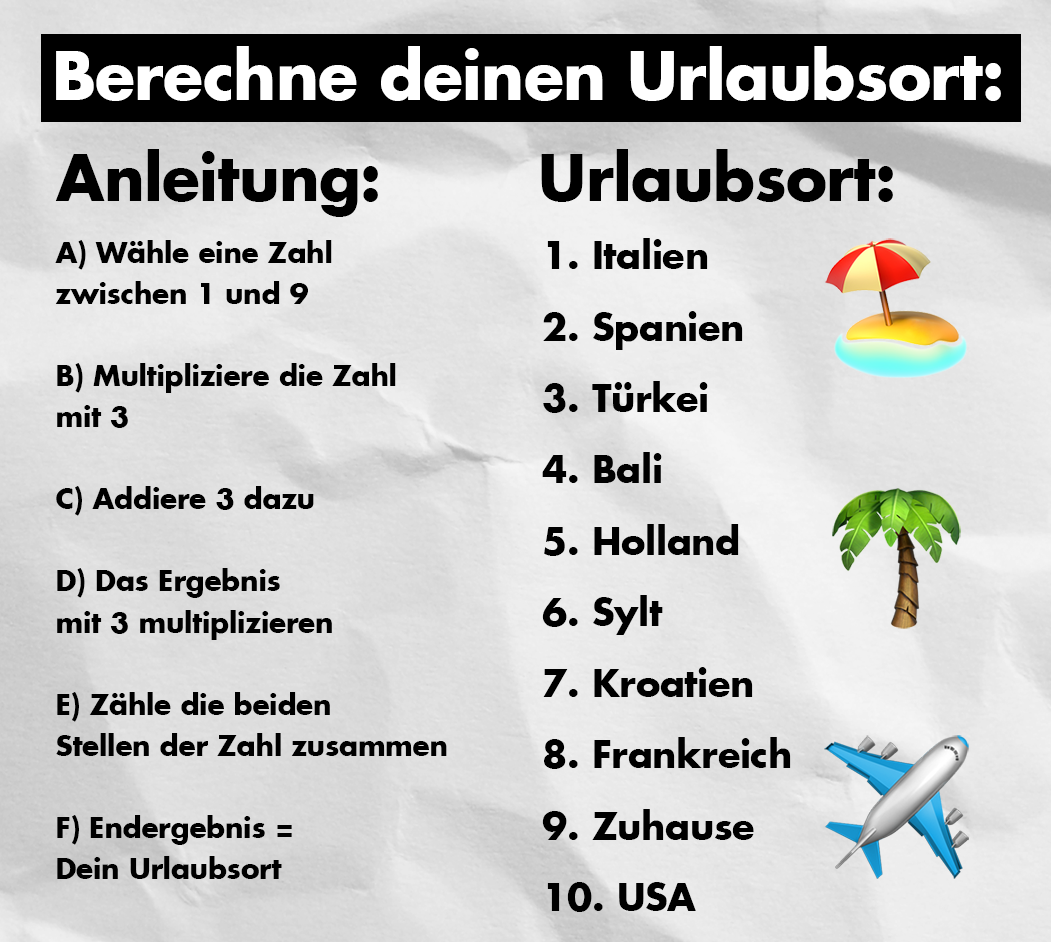
\includegraphics[width=0.5\textwidth]{urlaubsort.png}
\end{center}
Lies eine Zahl zwischen 1 und 9 ein und gib auf der Konsole \emph{deinen nächsten Urlaubsort} aus. 
\end{frame}


\begin{frame}<beamer:0>[fragile]
\frametitle{Lösung}
\begin{solutionblock}{Urlaubsort}
\begin{minted}{python}
number = input("Gib eine Zahl zwischen 1 und 9 ein: ")
number = int(number)

number = number * 3
number = number + 3
number = number * 3

cross_sum = number // 10 + number % 10
print("Dort verbringst Du Deinen Urlaub: ")
if cross_sum == 1:
  print("Italien")
elif cross_sum == 2:
  print("Spanien")
# ... more elif statements ... 
elif cross_sum == 9:
  print("Zu Hause")
else:
  print("USA")
\end{minted}
\end{solutionblock}
\end{frame}



\begin{fragile}{}
\begin{block}{Der \emph{Ternary Operator}}
\vspace{2pt}
Oftmals möchte man eine Variable in Abhängigkeit eines Wahrheitswertes definieren. Für diesen einfachen Fall, ist das \pybw{if-else}-Konstrukt sehr umständlich. Stattdessen kann man für die Kürze den \emph{ternary operator} verwenden. 
\end{block}
\vspace{12pt}
\pause
\begin{exampleblock}{Beispiel}
	\vspace{2pt}
	\begin{minted}{python}
	if x < 0: 
	  sign = "negative"	
	else: 
	  sign = "positive"
	\end{minted}
\end{exampleblock}
\pause 
\begin{block}{Stattdessen mit Ternary Operator}
	\vspace{2pt}
	\py{sign = "negative" if x < 0 else "positive"}
\end{block}
\end{fragile}

\begin{fragile}[Übung]

\begin{block}{Ternary Operator}
	\vspace{2pt}
Lies eine ganze Zahl ein und gib ihren Betrag auf der Konsole aus. Schaffst Du es, das Ganze mit weniger als 5 Zeilen Code zu programmieren? 
\end{block}

\vspace{12pt}

\begin{solutionblock}<beamer:0>{Lösung}
\begin{minted}{python}
x = input("Gib eine Zahl ein: ")
x = float(x)
abs_value = x if x >= 0 else -x
print(f"Der Betrag von {x} ist {abs_value}")
\end{minted}
\end{solutionblock}

\end{fragile}





\section{Die For-Schleife \\ \footnotesize Einen Programmabschnitt x-mal ausführen}




\begin{frame}

\begin{block}{Problemstellung}
\vspace{2pt}
Lies eine ganze Zahl \py{x} ein. Gib dann folgende Zeilen auf der Konsole aus 

\texttt{1}\\
\texttt{2}\\
\texttt{3}\\
\texttt{4}\\
\vdots \\
\texttt{x}

\vspace{12pt}
Wie macht man das? 

\end{block}
\end{frame}

\begin{fragile}{}
	\begin{block}{Lösung \footnotesize (fast)}
		\begin{minted}{python}
			x = input("Gib eine Zahl ein")
			x = int(x)
			
			for k in range(1, x):	
			  print(k)
		\end{minted}
	\end{block}
\end{fragile}

\begin{frame}

	\renewcommand{\baselinestretch}{1.5}
	\metroset{block=fill}
	\begin{block}{Struktur der \texttt{for...in} Schleife}
		\vspace{2pt}
		\pause \py{for} \pause \textit{Variable} \pause \py{in} \pause \py{range}(\textit{start}, \textit{end})\pause\texttt{:} \pause \\
		\spacechar\spacechar Codezeile 1 \pause \\ 
\spacechar\spacechar Codezeile 2 \pause \\
\spacechar\spacechar \phantom{Code} \vdots \pause  \\
\textit{Code, der nicht mehr Teil der Schleife ist}
	\end{block}

\vspace{12pt}
\pause 

\metroset{block=transparent}
	\renewcommand{\baselinestretch}{1}
	\begin{block}{Wie funktioniert's?}
		\vspace{2pt}
	Die Schleifenvariable wird zunächst gleich dem unteren Wert in \py{range} gesetzt. Dann wird der \pybw{for}-Block wiederholt ausgeführt. Bei jedem Durchgang wird die Schleifenvariable um \pybw{1} vergrößert und zwar so lange, wie der Wert der Schleifenvariable kleiner als der obere Wert in \py{range} ist. 	
	\end{block}
\end{frame}

\begin{fragile}
\begin{exampleblock}{Beispiel}
\vspace{2pt}
	
	\begin{overprint}
		\onslide<1|handout:0>
\begin{minted}{python}
for x in range(1,5)
  print(2*x)
\end{minted}
\onslide<2|handout:1>
\begin{minted}{python}
for x in range(1,5)
  print(2*x)

# prints 
# 2
# 4
# 6
# 8
\end{minted}
\end{overprint}
\end{exampleblock}
\end{fragile}


\begin{frame}
\begin{block}{Good to know}
	\pause
	\begin{itemize}[<+->]
		\item Achtung: Die Schleifenvariable erreicht nie das obere Ende der \py{range}-Funktion, sondern bleibt immer \pybw{1} drunter. 
		\item Die \py{range}-Funktion ist nicht auf 1er-Schrittweite beschränkt. Mit folgendem Ausdruck werden die Zahlen von \py{0} bis \py{9} z.B. in 3er-Schritten durchlaufen: \py{range(0, 10, 3)}. 
		\item \texttt{For}-Schleifen sind flexibel und können alles mögliche durchlaufen, z.B. auch die einzelnen Buchstaben eines Strings (dazu später mehr).
	\end{itemize}
\end{block}
\end{frame}


\begin{fragile}[Übung zum Einstieg]
	
\begin{block}{Eingangsbeispiel}
\vspace{2pt}
Schreibe ein Skript, das alle Zahlen von 1 bis 100 auf der Konsole ausgibt. 

\vspace{12pt}
\begin{solutionblock}{Lösung}
\begin{minted}{python}
for k in range(1, 101)
  print(k)
\end{minted}
\end{solutionblock}
\end{block}
\end{fragile}



\begin{fragile}[Übungen]

\begin{block}{Zählen}
\vspace{2pt}
Zähle auf der Konsole in 7-er Schritten bis 70.

\console{7} \\
\console{14} \\
\phantom{|} \vdots\\
\console{70}
\end{block}


\pause 

\vspace{12pt}

\begin{block}{Einmaleins: Die 7er-Reihe}
	\vspace{2pt}
	Schreibe ein kleines Skript, was die 7er-Reihe (bis 70) wie folgt auf der Konsole ausgibt: 
	
	\console{1 mal 7 ist 7}\\	
	\console{2 mal 7 ist 14}\\
	\phantom{4 mal} \vdots  
\end{block}
\end{fragile}


\begin{frame}<beamer:0>[fragile]{Lösungen}


\begin{solutionblock}{Zählen}
\begin{minted}{python}
for k in range(1, 11):
  print(7*k)
\end{minted}
\end{solutionblock}

\vspace{12pt}

\begin{solutionblock}{Einmaleins}
\begin{minted}{python}
for k in range(1, 11):
  print(f"{k} mal 7 ist {7 * k}")
\end{minted}
\end{solutionblock}

\end{frame}

\begin{fragile}[Komplexe Übungen]

\begin{block}{Zählen in krummen Abständen}	
\vspace{2pt}
Zähle auf der Konsole bis 20, allerdings sollen nur Zahlen ausgegeben werden, die durch 3 oder durch 5 teilbar sind:

\console{3} \\
\console{5} \\
\console{6} \\
\console{9} \\
\console{10}\\
\phantom{|}\vdots\\
\console{20}
\end{block}

\vspace{12pt}
\pause

\begin{block}{Anzahl bestimmen}
\vspace{2pt}
Bestimme die Anzahl der Zahlen zwischen 1 und 20, die durch 3 oder durch 5 teilbar sind. 
\end{block}
\end{fragile}

\begin{frame}<beamer:0>[fragile]{Lösungen}


\begin{solutionblock}{Zählen in krummen Abständen}
\begin{minted}{python}
for k in range(1, 21):
  if k % 3 == 0 or k % 5 == 0: 
    print(k)
\end{minted}
\end{solutionblock}

\vspace{12pt}

\begin{solutionblock}{Anzahl bestimmen}
\begin{minted}{python}
counter = 0
for k in range(1, 21):
  if k % 3 == 0 or k % 5 == 0:
    counter = counter + 1 
print(f"Es gibt {counter} gesuchte Zahlen")
\end{minted}
\end{solutionblock}

\end{frame}


\begin{fragile}[Schwierigere Übungen]
	
\begin{block}{Das Gauss-Problem}
\vspace{2pt}	
Berechne die Summe der Zahlen 1 bis 100. 
\end{block}
\vspace{12pt}
\begin{solutionblock}{Lösung}
\begin{minted}{python}
result = 0
for k in range(1, 101):
  result = result + k
print(f"Das Ergebnis ist {result}.")
\end{minted}
\end{solutionblock}

	
	
\end{fragile}


\begin{fragile}[Übung]
\begin{block}{Schleife über einen String}
\vspace{2pt}
Lies Deinen Namen auf der Konsole ein und gib die Buchstaben einzeln auf der Konsole auf. 
\end{block}
\vspace{12pt}
\begin{solutionblock}{Lösung}
\begin{minted}{python}
name = input("Gib Deinen Namen ein: ")

for letter in name:
  print(letter)
\end{minted}
\end{solutionblock}
\end{fragile}




\begin{fragile}[Übung]
\begin{block}{Needle-Haystack-Problem}
\vspace{2pt}
Lies Deinen Namen auf der Konsole ein und überprüfe, ob er den Buchstaben \emph{a} (groß/klein) enthält. 
\end{block}
\vspace{12pt}
\begin{solutionblock}{Lösung}
\begin{minted}{python}
name = input("Gib ein Wort ein: ")

# Flag (Schalter) initialisieren
name_contains_letter_a = False

for letter in name:
  if letter == "a" or letter == "A":
    name_contains_letter_a = True

if name_contains_letter_a:
  print("Der Name enthält ein 'a'.")
else:
  print("Der Name enthält kein 'a'.")
\end{minted}
\end{solutionblock}
\end{fragile}



\begin{fragile}[Übung mit Trick]
\begin{block}{Quersumme}
	\vspace{2pt}
	Lies eine ganze Zahl \py{x} ein und bestimme ihre Quersumme. 
	
	\textbf{Tipp:} Wandle die Zahl zunächst in einen String um \\
\end{block}

\vspace{12pt}

\begin{solutionblock}{Lösung}
\begin{minted}{python}
number = input("Gib eine Zahl ein: ")
result = 0
# Wir lassen die Zahl als String, damit wir eine Schleife über die Ziffern legen können
for digit in number:
  result = result + int(digit)  # Achtung: digit ist ja eigentlich ein String

print(f"Die Quersumme von {number} ist {result}")
\end{minted}
\end{solutionblock}

\end{fragile}


\begin{fragile}[Brutale Übung]
	
	
\begin{block}{Fibonacci-Zahlen}
\vspace{2pt}
Die Zahlenfolge $1,1,2,3,5,8,13\ldots$ nennt man \emph{Fibonacci}-Folge. Dabei ensteht ein Element der Folge, durch die Addition des vorherigen und vorvorherigen Elements. 

\vspace{1pt}

Berechne die 30. Fibonacci-Zahl.  
\end{block}
\vspace{12pt}
\begin{solutionblock}{Lösung}
\begin{minted}{python}
last = 1  # letzte Zahl
current = 1  # aktuelle Zahl

for k in range(2, 31):
  old_current = current  # Zahl zwischenspeichern
  current = current + last
  last = old_current

print(f"Die {k}-te Fibonacci-Zahl ist {current}")
\end{minted}
\end{solutionblock}
	
\end{fragile}










	





\section{Die While-Schleife \\ \footnotesize Wie die For-Schleife nur abstrakter und open-end}

\begin{frame}
\begin{block}{Problemstellung}
	\vspace{2pt}
	Lies immer wieder eine Zahl von der Konsole ein. Höre auf, wenn diese Zahl 7 ist. 
	
	Wie macht man das? 
\end{block}
\end{frame}

\begin{fragile}
	
\begin{block}{Lösung}
		\vspace{2pt}
		
	\begin{minted}{python}
		x = 0
		
		while x != 7: 
		  x = input("Gib eine Zahl an: ")
		  x = int(x)
		  
		print("Fertig!")
	\end{minted}
	
\end{block}
\end{fragile}

\begin{frame}

\renewcommand{\baselinestretch}{1.5}
\metroset{block=fill}
\begin{block}{Struktur der \texttt{while}-Schleife}
	\vspace{2pt}
	\pause \py{while} \pause \textit{Bedingung}\pause\texttt{:} \pause \\
	\spacechar\spacechar Codezeile 1 \pause \\ 
	\spacechar\spacechar Codezeile 2 \pause \\
	\spacechar\spacechar \phantom{Code} \vdots \pause  \\
	\textit{Code, der nicht mehr Teil der Schleife ist}
\end{block}
\vspace{12pt}
\pause 
\metroset{block=transparent}
\renewcommand{\baselinestretch}{1}
\begin{block}{Wie funktioniert's?}
	\vspace{2pt}
	Die Schleife wird solange ausgeführt, solange die \emph{Bedingung} \py{True} ergibt. Nach jedem Durchgang wird der Ausdruck der \emph{Bedingung} neu ausgewertet. 
	Ist die Bedingung \py{False} wird der Code unterhalb des Schleifenblocks ausgeführt. 
\end{block}

\end{frame}

\begin{frame}
\begin{alertblock}{Achtung Endlosschleife}
	\vspace{2pt}
	Man sollte immer darauf achten, dass die Bedingung in der \pybw{while}-Schleife auch wirklich irgendwannmal \py{False} wird. Ansonsten bleibt das Programm in einer \emph{Endlosschleife} gefangen. 
\end{alertblock}
\end{frame}

\begin{fragile}[Übung]

\begin{block}{Ersetze eine \pybw{for}-Schleife durch eine \pybw{while}-Schleife}
\vspace{2pt}
Schreibe ein Skript, das alle Zahlen von 1 bis 100 auf der Konsole ausgibt. Verwende eine While-Schleife.
\vspace{12pt}
\begin{solutionblock}{Lösung}
\begin{minted}{python}
k = 1
while k <= 100:
  print(k)
  k += 1
\end{minted}
\end{solutionblock}
\end{block}
\end{fragile}


\begin{fragile}[Übung]
\begin{block}{Quizfrage}
\vspace{2pt}
Schreibe ein Programm, dass solange nach einer Hauptstadt Deiner Wahl fragt, bis die richtige Antwort eingegeben wird. 
\end{block}

\pause 
\vspace{12pt}

\begin{exampleblock}{Beispiel}
\vspace{2pt}


\console{Was ist die Hauptstadt von Frankreich?}

Darauf hin soll entsprechend der Antwort folgendes Feedback auf der Konsole erscheinen: 

\console{Das war richtig!} 

bzw. 

\console{Das war falsch! Versuch's gleich nochmal}
\end{exampleblock}
	
\end{fragile}


\begin{frame}<beamer:0>[fragile]
\frametitle{Lösung}
\begin{solutionblock}{Quizfrage}
\begin{minted}{python}
answer = input("Was ist die Hauptstadt von Frankreich?")
while answer != "Paris": 
  print("Das war leider falsch, versuch es gleich nochmal")
  answer = input("")
print("Das war richtig!")
\end{minted}
\end{solutionblock}
\end{frame}


\begin{frame}{Übung}

\begin{block}{Ratespiel}
\vspace{2pt}
Definiere eine positive ganze Zahl \py{number_to_guess}. Der User kann nun wiederholt eine Zahl eingeben. Das Spiel endet, wenn die eingegebene Zahl mit \py{number_to_guess} übereinstimmt. 
Andernfalls wird auf der Konsole beispielsweise ausgegeben: 

\console{Sorry, Deine eingegebene Zahl war zu klein, versuche es nochmal: }

\pause
\textbf{Zusatz 1:} \\
Am Ende soll die Anzahl der Versuche angegeben werden.


\pause
\textbf{Zusatz 2:} \\
Google, wie Python die Zahl \py{number_to_guess} zufällig erzeugen kann (das verbessert das Gameplay).  

\end{block}
\end{frame}



\begin{frame}<beamer:0>[fragile]
\frametitle{Lösung}
\begin{solutionblock}{Ratespiel ohne Zusätze}
\begin{minted}{python}
number_to_guess = 512
guess = input("Rate meine Zahl: ")
guess = int(guess)

while guess != number_to_guess:
  if guess < number_to_guess:
    print("Deine Zahl war zu klein")
  else:
    print("Deine Zahl war zu groß")
  guess = input("Versuch's nochmal: ")
  guess = int(guess)

print("Du hast gewonnen")
\end{minted}
\end{solutionblock}
\end{frame}


\begin{frame}<beamer:0>[fragile]
\frametitle{Lösung}
\begin{solutionblock}{Ratespiel mit Zusatz 1}
\begin{minted}{python}
number_to_guess = 512
guess = input("Rate meine Zahl: ")
guess = int(guess)
counter = 1

while guess != number_to_guess:
  if guess < number_to_guess:
    print("Deine Zahl war zu klein")
  else:
    print("Deine Zahl war zu groß")
  guess = input("Versuch's nochmal: ")
  guess = int(guess)
  counter = counter + 1
  
print(f"Du hast nach {counter} Versuchen gewonnen")	
\end{minted}
\end{solutionblock}
\end{frame}






\begin{frame}<beamer:0>[fragile]
\frametitle{Lösung}
\begin{solutionblock}{Ratespiel mit Zusatz 2}
\begin{minted}{python}
import random 

number_to_guess = random.randint(1, 1000)
guess = input("Rate meine Zahl: ")
guess = int(guess)
# ... usw. 
\end{minted}
\end{solutionblock}
\end{frame}







\section{Den Schleifenfluss kontrollieren  \\ \footnotesize \texttt{break}, \texttt{continue} und \texttt{else}}


\begin{fragile}
	
\metroset{block=fill}

\begin{block}{Das \texttt{break}-Statement}
Taucht innerhalb einer Schleife das Schlüsselwort \py{break} auf, so wird die weitere Abarbeitung der Schleife abgebrochen. Die Ausführung wird mit dem Code \emph{nach} dem Schleifenblock ausgeführt. 		
\end{block}

\metroset{block=transparent}

\vspace{12pt} \pause 


\begin{exampleblock}{Beispiel}
\vspace{2pt}

\begin{overprint}
	\onslide<2|handout:0>
\begin{minted}{python}
for k in range(1,100):
  print(k)
  if k > 3:
    break
print("fertig")
\end{minted}
\onslide<3|handout:1>
\begin{minted}{python}
for k in range(1,100):
  print(k)
  if k > 3:
    break
print("fertig")
# 1 2 3 4 
# fertig
\end{minted}
\end{overprint}

\end{exampleblock}

	
\end{fragile}



\begin{fragile}
	
\metroset{block=fill}

\begin{block}{Das \texttt{continue}-Statement}
Taucht innerhalb einer Schleife das Schlüsselwort \py{continue} auf, so wird der aktuelle Schleifendurchgang abgebrochen. Die Ausführung wird mit der nächsten Schleifeniteration fortgesetzt. 
\end{block}

\metroset{block=transparent}

\vspace{12pt} \pause 


\begin{exampleblock}{Beispiel}
\vspace{2pt}

\begin{overprint}
\onslide<2|handout:0>
\begin{minted}{python}
for k in range(1,11):
  if k % 2 == 0:
    continue
  print(k)
\end{minted}
\onslide<3|handout:1>
\begin{minted}{python}
for k in range(1,11):
  if k % 2 == 0:
    continue
  print(k)
# 1 3 5 7 9 
\end{minted}
\end{overprint}
\end{exampleblock}
	
	
\end{fragile}


\begin{fragile}
	
\metroset{block=fill}

\begin{block}{Der \texttt{else}-Block einer Schleife}
Analog zum \py{if}-Statement, kann auch eine Schleife einen \py{else}-Block haben. Dieser wird ausgeführt, wenn die Schleife \emph{regulär} (also nicht durch die Verwendung von \py{break}) beendet wird.  
\end{block}

\metroset{block=transparent}

\vspace{12pt} \pause 


\begin{exampleblock}{Beispiel}
\begin{minted}{python}
name = input("Dein Name: ")

for letter in name: 
  if letter == "a" or letter == "A":
    print("Dein Name enthält ein A")
    break
else: 
  print("Dein Name enthält kein A")
\end{minted}
\end{exampleblock}
	
	
\end{fragile}



\begin{fragile}[Übungen]

\begin{block}{Zählen bis zur nächsten 10er-Zahl}
	\vspace{2pt}
Lies eine Zahl \pybw{x} ein und gib auf der Konsole die Zahlen von \pybw{x} bis zur nächsten 10er-Zahl aus. 
\\
Ist die Eingabe \pybw{x = 17}, so soll die Ausgabe wie folgt aussehen: 

\console{17}\\
\console{18}\\
\console{19}\\
\console{20}
\end{block}
	
\vspace{12pt}
\pause 

\begin{block}{Zählen mit Lücken}
	\vspace{2pt}
	Schreibe ein Skript, dass die Zahlen von 1 bis 99 aufzählt, dabei allerdings die 10er-Zahlen weglässt. Verwende dabei ein \pybw{continue}-Statement.
\end{block}
\end{fragile}

\begin{frame}<beamer:0>[fragile]{Lösungen}

\begin{solutionblock}{Zählen bis zur nächsten 10er-Zahl}
\begin{minted}{python}
x = input("Gib eine Zahl an: ")
x = int(x)

for k in range(x, x + 11):
  print(k)
  if k % 10 == 0:
    break
\end{minted}
\end{solutionblock}

\vspace{12pt}

\begin{solutionblock}{Zählen mit Lücken}
\begin{minted}{python}
for k in range(1, 100):
  if k % 10 == 0:
    continue
  print(k)
\end{minted}
\end{solutionblock}

\end{frame}

\begin{fragile}[Übung]
\begin{block}{Quizfrage mit Ausstiegsmöglichkeit}
\vspace{2pt}
Schreibe ein Programm, dass solange nach einer Hauptstadt Deiner Wahl fragt, bis die richtige Antwort eingegeben wird. Wird allerdings der Buchstabe \pybw{q} eingegeben, so bricht das Programm ab. 

\vspace{12pt}

\begin{solutionblock}{Quizfrage mit Ausstiegsmöglichkeit}
\begin{minted}{python}
answer = input("Was ist die Hauptstadt von Frankreich?")
while answer != "Paris": 
  print("Das war leider falsch, versuch es gleich nochmal")
  answer = input("")
  if answer == "q": 
    break
else: 
  print("Das war richtig!")
\end{minted}
\end{solutionblock}
\end{block}
\end{fragile}




\begin{fragile}[Harte Übung]
\begin{block}{Primzahltest}
\vspace{2pt}
Lies eine ganze Zahl \py{x} ein und überprüfe, ob diese Zahl eine Primzahl ist. Die Ausgabe des Programms soll etwa wie folgt aussehen:  

\console{Die Zahl 28061983 ist eine Primzahl.}
\end{block}

\vspace{12pt}
\begin{solutionblock}{Lösung}
\begin{minted}{python}
x = input("Gib eine Zahl ein: ")
x = int(x)

for k in range(2, x):
  if x % k == 0:
    print(f"{x} ist keine Primzahl.")
    break
else:
  print(f"{x} ist eine Primzahl.")
\end{minted}
\end{solutionblock}

\end{fragile}



\section{Listen \\ \footnotesize Viele Variablen gleichzeitig speichern}


\begin{frame}
\begin{block}{Problemstellung}
\vspace{2pt}
Lies mit Hilfe einer Schleife nach und nach Ländernamen ein. 
Alle Länder sollen dabei gespeichert werden. Danach sollst Du die Möglichkeit haben, das soundsovielte Land anzeigen lassen zu können.   

\vspace{8pt}

Wie macht man das? 
\end{block}
\end{frame}

\begin{fragile}{}
\begin{block}{Lösung \footnotesize(fast)}
\begin{minted}{python}
# ...
# Um das Eingaben der Länder kümmern wir uns noch 
countries = ["Deutschland", "Frankreich", "Italien", "Spanien"] 

index = input("Das wievielte Land möchtest Du nocheinmal anschauen?")
index = int(index)

print(f"Das { index }. Land ist { countries[index] }")
\end{minted}
\end{block}
\end{fragile}


\begin{fragile}

\metroset{block=fill}
\begin{block}{Struktur einer \emph{Liste}}
\vspace{2pt}
\large
\texttt{my\_list = }\pause {\Large\texttt{[}}\pause 
\texttt{element\_0}\pause,
\pause 
\texttt{element\_1}, \pause 
 \dots   
, \texttt{element\_n}\pause \Large{\texttt{]}}
\end{block}

\pause 

Die Variable \py{my_list} trägt nicht nur einen Wert, sondern $n+1$ Werte. Ansonsten verhält sich \py{my_list} wie eine ganz \enquote{normale} Variable. 
Als Einträge einer Liste sind beliebige Werte mit beliebigen Datentypen zugelassen. 


\vspace{12pt}

\pause

\textbf{Frage:} Welchen Datentyp hat die Liste \py{[2, 2.3, "Hello"]} ? 
	
\end{fragile}

\begin{frame}
	
\begin{block}{Auf Listenelemente zugreifen}
	
\vspace{2pt}

Auf das \pybw{n}-te Element der Liste \py{my_list} kann man mittels \py{my_list[n]} zugreifen. 

\pause 

Mit \py{my_list[-1]}, \py{my_list[-2]}, etc. kann man auf das letzte, vorletzte, etc. Element 
der Liste zugreifen. 

\end{block}

\pause 
\vspace{12pt}

\begin{alertblock}{Achtung}
\vspace{2pt}
Python fängt bei 0 an zu zählen. D.h. das erste Element in der Liste hat den Index 0. \\
Beispiel: \py{my_list[1]} liefert das \textbf{2. Element} der Liste. 
\end{alertblock}

	
\end{frame}	


\begin{frame}
\begin{block}{Schreibzugriff auf Listenelemente}
\vspace{2pt}
Nach dem gleichen Prinzip lassen sich einzelne Listeneinträge verändern. \\
Beispiel: \py{my_list[3] = "Albanien"}. 
\end{block}

\pause 
\vspace{12pt}



\begin{alertblock}{Achtung}
\vspace{2pt}
Man kann nur schon existierende Listeneinträge verändern. 
\end{alertblock}

\pause 
\vspace{12pt}

\end{frame}


\begin{frame}
\begin{block}{Listeneinträge hinzufügen}
	\vspace{2pt}
	Mit der \emph{Methode} \pybw{.append()} kann ein Eintrag zur Liste hinzugefügt werden. \\ 
	Bsp: \py{my_list.append("Russland")} fügt den String \py{"Russland"} zu der Liste hinzu. 
\end{block}	

\pause 
\vspace{12pt}


\begin{block}{Listeneinträge entfernen}
	\pause 
\vspace{2pt}
Mit dem Keyword \pybw{del} kann man Einträge an einer bestimmten Position löschen. Dabei verschieben sich die darauffolgenden Einträge um \pybw{1} nach vorne. \\
Beispiel: \py{del my_list[2]} löscht das dritte Element.  

\pause 

Mit der Methode \pybw{.remove()} kann man Einträge mit einem bestimmten Wert löschen. \\
Beispiel: \py{my_list.remove("Italien")} entfernt den ersten Eintrag mit dem Wert \py{"Italien"}. Ist der Wert nicht vorhanden gibt es eine Fehlermeldung. 
\end{block}
\end{frame}

\begin{fragile}[Übung]
\begin{block}{Eine Liste erstellen}
\vspace{2pt}
Schreibe ein kleines Programm, dass Dich ca. 4x nach einem Land fragt, das Du besucht hast und Dir am Ende die Liste der besuchten Länder ausgibt. 	
\end{block}
\vspace{12pt}
\begin{solutionblock}{Lösung}
\begin{minted}{python}
countries = []
for k in range(1, 5):
  country = input("Wo warst Du schonmal im Urlaub? ")
  countries.append(country)
print(countries)
\end{minted}
\end{solutionblock}
\end{fragile}





\begin{fragile}[Übung]
\begin{block}{Das Eingangsproblem}
\vspace{2pt}
Schreibe ein kleines Programm, dass solange Namen von Ländern einliest, bis Du \textbf{q} drückst. Danach sollst Du die Möglichkeit haben, eine Zahl \pybw{k} einzugeben, so dass das  \pybw{k}-te Land angezeigt wird. 
\end{block}	
\end{fragile}

\begin{frame}<beamer:0>[fragile]{Lösung}
\begin{solutionblock}{Das Eingangsproblem}
\begin{minted}{python}
countries = []
while True:
  country = input("Gib ein Land ein: ")
  if country == "q":
    break
  countries.append(country)

index = input("Das wievielte Land möchtest Du nochmal anschauen?")
index = int(index)
print(f"Das { index }. Land ist { countries[index-1] }.")
\end{minted}
\end{solutionblock}
\end{frame}








\begin{frame}
\begin{block}{Mutability}

\vspace{2pt}
Listen sind der erste Datentyp, den wir kennenlernen, der \emph{mutable} (veränderbar) ist. Die bisherigen Datentypen waren \emph{immutable}, d.h. man konnte sie zwar überschreiben, aber nicht verändern. 
\end{block}

\pause 
\vspace{12pt}

\metroset{block=fill}
\begin{block}{Call by Reference vs. Call by Value}
\vspace{2pt}
Enthält die Variable \py{my_list} eine Liste, so speichert Python eigentlich gar nicht die Liste in dieser Variable, sondern nur die Speicheradresse der Liste. 
Dieses vorgehen nennt man auch \emph{Call by Reference}. Bei den Datentypen \py{int} und \py{str} wird stattdessen tatsächlich der Wert der Variable abgespeichert. Dies nennt man \emph{Call by Value}.

\end{block}
\end{frame}

\begin{fragile}[Übung]
\begin{block}{Eine Liste kopieren}
\vspace{2pt}
Definiere die Variable \py{my_list} als die Liste \py{[1,2,3]}. Kopiere die Variable \py{my_list} in die Variable \py{my_list_copy}. Füge einen weiteren Eintrag zu \py{my_list} hinzu. Welchen Wert hat \py{my_list_copy}? 
\end{block}
\vspace{12pt}
\begin{solutionblock}{Lösung}
\begin{minted}{python}
my_list = [1, 2, 3]
my_list_copy = my_list
my_list.append(4)
print(my_list_copy) # 1 2 3 4 
\end{minted}
\end{solutionblock}
\end{fragile}



\begin{fragile}
\begin{block}{Schleife über Liste}
\vspace{2pt}
Analog wie über Strings und Ranges kann man Schleifen auch über eine Liste laufen lassen.  
\end{block}
\vspace{12pt}
\pause 

\begin{exampleblock}{Beispiel}
\vspace{2pt}
\begin{overprint}
\onslide<2|handout:0>
\begin{minted}{python}
countries = ["Bulgarien", "Griechenland", "Türkei", "Libanon"]

for country in countries:
  print(country)
\end{minted}
\onslide<3|handout:1>
\begin{minted}{python}
countries = ["Bulgarien", "Griechenland", "Türkei", "Libanon"]

for country in countries:
  print(country)
  
# Bulgarien
# Griechenland
# Türkei
# Libanon
\end{minted}
\end{overprint}
\end{exampleblock}
\end{fragile}


\begin{fragile}
\begin{block}{Schleife über Liste mit Indizes}
\vspace{2pt}
Möchte man in einer Schleife nicht nur die Listeneinträge, sondern auch die Indizes verwenden, so muss man die Funktion \py{enumerate()} auf die Liste anwenden. 
\end{block}
\vspace{12pt}
\pause 

\begin{exampleblock}{Beispiel}
\vspace{2pt}
\begin{overprint}
\onslide<2|handout:0>
\begin{minted}{python}
countries = ["Guatemala", "Nicaragua", "Honduras", "Belize"]

for (index, country) in enumerate(countries):
  print(f"Das {index + 1}. Land ist {country}")
\end{minted}
\onslide<3|handout:1>
\begin{minted}{python}
countries = ["Guatemala", "Nicaragua", "Honduras", "Belize"]

for (index, country) in enumerate(countries):
  print(f"Das {index + 1}. Land ist {country}")

# Das 1. Land ist Guatemala
# Das 2. Land ist Nicaragua
# Das 3. Land ist Honduras
# Das 4. Land ist Belize
\end{minted}
\end{overprint}
\end{exampleblock}
\end{fragile}


\begin{frame}{Übung}

\begin{block}{Liste durchsuchen}
	\vspace{2pt}
Prüfe, ob in einer Liste von Ländern das Land \py{"Italien"} vorkommt. Gib dazu auf der Konsole entweder 

\console{Italien ist in der Liste}

oder 

\console{Italien ist nicht in der Liste}

aus.  

\end{block}
\end{frame}


\begin{frame}<beamer:0>[fragile]{Lösung}
\begin{solutionblock}{Liste durchsuchen}
\begin{minted}{python}
# Wähle ein Beispiel für countries
countries = ["Finnland", "Norwegen", "Schweden", "Dänemark"]

for country in countries:
  if country == "Italien":
    print("Italien ist in der Liste")
    break
else: 
  print("Italien ist nicht in der Liste")
\end{minted}
\end{solutionblock}
\end{frame}

\begin{fragile}

\begin{block}{Ist ein Element in einer Liste enthalten?}
\vspace{2pt}	
Möchte man prüfen, ob ein Element in einer Liste enthalten ist, so kann man auch das Schlüsselwort \py{in} verwenden. 
\end{block}

\pause 
\vspace{12pt}

\begin{exampleblock}{Beispiel}
\vspace{2pt}
\begin{overprint}
\onslide<2|handout:0>
\begin{minted}{python}
countries = ["Finnland", "Norwegen", "Schweden", "Dänemark"]

var_1 = "Finnland" in countries
var_2 = "Deutschland" in countries

print(var_1)  
print(var_2)
\end{minted}
\onslide<3|handout:1>
\begin{minted}{python}
countries = ["Finnland", "Norwegen", "Schweden", "Dänemark"]

var_1 = "Finnland" in countries
var_2 = "Deutschland" in countries

print(var_1)  # True
print(var_2)  # False
\end{minted}
\end{overprint}

\end{exampleblock}
\end{fragile}


\begin{fragile}
	
\begin{block}{Eine Liste sortieren}
\vspace{2pt}
Um eine Liste zu sortieren, verwende die Methode \pybw{.sort()}. Dies verändert die Liste dauerhaft. \\
\pause 
Um eine sortierte Kopie einer Liste zu erstellen, verwende die Funktion \pybw{sorted()}.  \\
\pause 
Mit Hilfe des Parameters \pybw{reverse=True} lässt sich eine Liste absteigend ordnen. 
\end{block}	

\pause \vspace{12pt}

\begin{exampleblock}{Beispiel für \texttt{sort}}
\vspace{2pt}
\begin{overprint}
\onslide<4|handout:0>
\begin{minted}{python}
my_list = [1, 5, 2, 7]
my_list.sort()
print(my_list)  
\end{minted}
\onslide<5-|handout:1>
\begin{minted}{python}
my_list = [1, 5, 2, 7]
my_list.sort()
print(my_list)  # [1, 2, 5, 7]
\end{minted}
\end{overprint}

\end{exampleblock}

\vspace{12pt}

\pause \pause 

\begin{exampleblock}{Beispiel für \texttt{sorted}}
\vspace{2pt}
\begin{overprint}
\onslide<6|handout:0>
\begin{minted}{python}
my_list = [1, 5, 2, 7]
sorted_list = sorted(my_list)
print(my_list)  
print(sorted_list)  
\end{minted}
\onslide<7|handout:1>
\begin{minted}{python}
my_list = [1, 5, 2, 7]
sorted_list = sorted(my_list)
print(my_list)  # [1, 5, 2, 7]
print(sorted_list)  # [1, 2, 5, 7]
\end{minted}
\end{overprint}
\end{exampleblock}
\end{fragile}

\begin{fragile}
\begin{exampleblock}{Beispiel für absteigende Sortierung}
\vspace{2pt}
\begin{overprint}
\onslide<1|handout:0>
\begin{minted}{python}
my_list = [1, 5, 2, 7]
my_list.sort(reverse=True)
print(my_list)  

my_list = [7, 12, 5, 18]
sorted_list = sorted(my_list, reverse=True)
print(sorted_list) 
\end{minted}
\onslide<2|handout:1>
\begin{minted}{python}
my_list = [1, 5, 2, 7]
my_list.sort(reverse=True)
print(my_list)  # [7, 5, 2, 1]

my_list = [7, 12, 5, 18]
sorted_list = sorted(my_list, reverse=True)
print(sorted_list) # [18, 12, 7, 5] 
\end{minted}
\end{overprint}
\end{exampleblock}
\end{fragile}


\begin{fragile}[Übung]
	
\begin{block}{Beste/Schlechteste Note}
\vspace{2pt}
Sei \py{grades} eine Liste der Noten deiner letzten Klausuren (z.B. \py{grades = [12, 9, 14, 11]}). 
Gib dann auf der Konsole einmal die beste und einmal die schlechteste Note aus. 
\end{block}	

\vspace{12pt}

\begin{solutionblock}{Lösung}
\begin{minted}{python}
grades = [12, 9, 14, 11]
grades.sort()
min_grade = grades[0]
max_grade = grades[-1]
print(f"Schlechteste Note: {min_grade}")
print(f"Beste Note: {max_grade}")
\end{minted}
\end{solutionblock}
\end{fragile}

\begin{fragile}
\begin{block}{Nützliche Funktionen/Methoden}
\vspace{2pt}	
Für Listen stellt Python viele nützliche Methoden bzw. Funktionen bereit. Wenn Du googlest, findest Du für viele \enquote{Alltagsfragen} eine Lösung. 

Zum Beispiel hier: \texttt{https://docs.python.org/3/tutorial/datastructures.html}
\end{block}

\pause
\vspace{12pt}


\begin{exampleblock}{Beispiele}
\begin{minted}{python}
my_list = [2, 4, 8, 1]

len(my_list)   # = 4  (Gibt die Anzahl der Elemente an)
sum(my_list)   # = 15 (Berechnet die Summe der Elemente)
my_list.reverse() # [1, 8, 4, 2] (Dreht die Reihenfolge um)
my_list.insert(2,-1) # [2, 4, -1, 8, 1] (fügt den Wert -1 an Position 2 ein)
my_list.pop() # 1 (Gibt den letzten Eintrag der Liste zurück und entfernt ihn aus der Liste)
\end{minted}
\end{exampleblock}
\end{fragile}


\begin{fragile}[Übung]

\begin{block}{Durchschnittsnote}
\vspace{2pt}
Sei \py{grades} wieder eine Liste mit deinen letzten Noten.  Gib auf der Konsole die Durchschnittsnote aus. 
\end{block}	

\vspace{12pt}

\begin{solutionblock}{Lösung}
\begin{minted}{python}
grades = [12, 9, 14, 11]
total_sum = sum(grades)
count = len(grades)
average = total_sum/count
print(f"Die Durchschnittsnote ist {average}")
\end{minted}
\end{solutionblock}
	
\end{fragile}

\begin{frame}
\begin{block}{Slicing}
\vspace{2pt}
Wenn man eine Liste hat, ist es oft nötig, einen Teil der Liste \enquote{auszuschneiden}.\\
\pause
Dafür hat Python die \emph{Slice-Notation} eingeführt. \\
\pause 
Diese funktioniert nach folgendem Schema: 

\pause  \py{my_list[start:stop:step]}. 

\pause 
Die Einträge (start, stop, step) sind dabei jeweils optional. Wie immer wird der obere Wert (\pybw{stop}) gerade nicht erreicht.  
\pause 


Slicing lässt sich übrigens auch nach dem gleichen Schema auch auf Strings anwenden. 
\end{block}	

\pause
\vspace{12pt}

\begin{alertblock}{Wichtig}
\vspace{2pt}
Wenn man Slicing anwendet, erhält man eine Kopie der ausgewählten Elemente zurück. Die ursprüngliche Liste wird \emph{nicht} verändert. 
\end{alertblock}
\end{frame}


\begin{fragile}
\begin{exampleblock}{Beispiele}
	\vspace{2pt}
\begin{overprint}
\onslide<1|handout:0>
\begin{minted}{python}
my_list = [2, 4, 6, 8, 10]

my_list[1:3]    
my_list[0:4]     
my_list[1:1]     
my_list[0:4:2]   
my_list[:3]      
my_list[2:]      
my_list[:]      
my_list[1:-2]    
my_list[-3:-1]  
my_list[::-1]    
\end{minted}

\onslide<2|handout:0>
\begin{minted}{python}
my_list = [2, 4, 6, 8, 10]

my_list[1:3]     # [4, 6]
my_list[0:4]     
my_list[1:1]     
my_list[0:4:2]   
my_list[:3]      
my_list[2:]     
my_list[:]       
my_list[1:-2]   
my_list[-3:-1]  
my_list[::-1]    
\end{minted}

\onslide<3|handout:0>
\begin{minted}{python}
my_list = [2, 4, 6, 8, 10]

my_list[1:3]     # [4, 6]
my_list[0:4]     # [2, 4, 6, 8]
my_list[1:1]     
my_list[0:4:2]   
my_list[:3]      
my_list[2:]      
my_list[:]       
my_list[1:-2]    
my_list[-3:-1]  
my_list[::-1]    
\end{minted}

\onslide<4|handout:0>
\begin{minted}{python}
my_list = [2, 4, 6, 8, 10]

my_list[1:3]     # [4, 6]
my_list[0:4]     # [2, 4, 6, 8]
my_list[1:1]     # []
my_list[0:4:2]   
my_list[:3]      
my_list[2:]     
my_list[:]       
my_list[1:-2]    
my_list[-3:-1]   
my_list[::-1]    
\end{minted}


\onslide<5|handout:0>
\begin{minted}{python}
my_list = [2, 4, 6, 8, 10]

my_list[1:3]     # [4, 6]
my_list[0:4]     # [2, 4, 6, 8]
my_list[1:1]     # []
my_list[0:4:2]   
my_list[:3]      
my_list[2:]      
my_list[:]       
my_list[1:-2]    
my_list[-3:-1]   
my_list[::-1]    
\end{minted}

\onslide<6|handout:0>
\begin{minted}{python}
my_list = [2, 4, 6, 8, 10]

my_list[1:3]     # [4, 6]
my_list[0:4]     # [2, 4, 6, 8]
my_list[1:1]     # []
my_list[0:4:2]   # [2, 6]
my_list[:3]      
my_list[2:]      
my_list[:]       
my_list[1:-2]    
my_list[-3:-1]   
my_list[::-1]    
\end{minted}

\onslide<7|handout:0>
\begin{minted}{python}
my_list = [2, 4, 6, 8, 10]

my_list[1:3]     # [4, 6]
my_list[0:4]     # [2, 4, 6, 8]
my_list[1:1]     # []
my_list[0:4:2]   # [2, 6]
my_list[:3]      # [2, 4, 6]
my_list[2:]      
my_list[:]       
my_list[1:-2]   
my_list[-3:-1]   
my_list[::-1]    
\end{minted}

\onslide<8|handout:0>
\begin{minted}{python}
my_list = [2, 4, 6, 8, 10]

my_list[1:3]     # [4, 6]
my_list[0:4]     # [2, 4, 6, 8]
my_list[1:1]     # []
my_list[0:4:2]   # [2, 6]
my_list[:3]      # [2, 4, 6]
my_list[2:]      # [6, 8, 10]
my_list[:]       
my_list[1:-2]    
my_list[-3:-1]  
my_list[::-1]    
\end{minted}

\onslide<9|handout:0>
\begin{minted}{python}
my_list = [2, 4, 6, 8, 10]

my_list[1:3]     # [4, 6]
my_list[0:4]     # [2, 4, 6, 8]
my_list[1:1]     # []
my_list[0:4:2]   # [2, 6]
my_list[:3]      # [2, 4, 6]
my_list[2:]      # [6, 8, 10]
my_list[:]       # [2, 4, 6, 8, 10]
my_list[1:-2]    
my_list[-3:-1]   
my_list[::-1]    
\end{minted}

\onslide<10|handout:0>
\begin{minted}{python}
my_list = [2, 4, 6, 8, 10]

my_list[1:3]     # [4, 6]
my_list[0:4]     # [2, 4, 6, 8]
my_list[1:1]     # []
my_list[0:4:2]   # [2, 6]
my_list[:3]      # [2, 4, 6]
my_list[2:]      # [6, 8, 10]
my_list[:]       # [2, 4, 6, 8, 10]
my_list[1:-2]    # [6]
my_list[-3:-1]    
my_list[::-1]     
\end{minted}

\onslide<11|handout:0>
\begin{minted}{python}
my_list = [2, 4, 6, 8, 10]

my_list[1:3]     # [4, 6]
my_list[0:4]     # [2, 4, 6, 8]
my_list[1:1]     # []
my_list[0:4:2]   # [2, 6]
my_list[:3]      # [2, 4, 6]
my_list[2:]      # [6, 8, 10]
my_list[:]       # [2, 4, 6, 8, 10]
my_list[1:-2]    # [6]
my_list[-3:-1]   # [6, 8] 
my_list[::-1]     
\end{minted}

\onslide<12|handout:1>
\begin{minted}{python}
my_list = [2, 4, 6, 8, 10]

my_list[1:3]     # [4, 6]
my_list[0:4]     # [2, 4, 6, 8]
my_list[1:1]     # []
my_list[0:4:2]   # [2, 6]
my_list[:3]      # [2, 4, 6]
my_list[2:]      # [6, 8, 10]
my_list[:]       # [2, 4, 6, 8, 10]
my_list[1:-2]    # [6]
my_list[-3:-1]   # [6, 8] 
my_list[::-1]    # [10, 8, 6, 4, 2]  
\end{minted}

\end{overprint}
\end{exampleblock}
\end{fragile}


\section{Dictionaries}

\begin{frame}
\begin{block}{Problemstellung}
\vspace{2pt}
Eine Variable soll nicht nur die Namen von Ländern enthalten, sondern auch noch deren Hauptstadt. 

\vspace{8pt}

Wie macht man das? 
\end{block}
\end{frame}

\begin{fragile}{}
\begin{block}{Lösung}
	\begin{minted}{python}
	capitals = {"Deutschland": "Berlin", "Spanien": "Madrid", "Italien": "Rom"}
	
	country = input("Von welchem Land möchtest Du die Hauptstadt wissen?")
	
	print(f"Die Hauptstadt von { country } ist { capitals[country] } Punkte")
	\end{minted}
\end{block}
\end{fragile}

\begin{fragile}
	
	\metroset{block=fill}
	\begin{block}{Struktur eines \emph{Dictionaries}}
		\vspace{2pt}
		\large
		\texttt{my\_dict = }\pause {\Large\texttt{\{}}\pause 
		\texttt{key\_1}\pause\texttt{:}\pause\texttt{value\_1}\pause,
		\pause 
		\texttt{key\_2:value\_2}, \pause 
		\dots   
		, \texttt{key\_n:value\_n}\pause \Large{\texttt{\}}}
	\end{block}
	\pause 
	
	Das \emph{Dictionary} \py{my_dict} enthält Schlüssel-Wert-Paare (\emph{key-value-pairs}). Die Schlüssel müssen eindeutig und unveränderlich sein (z.B. vom Typ \pybw{string} oder \pybw{int}). Die Werte dürfen beliebige Datentypen sein. 
	
\end{fragile}

\begin{fragile}

\begin{block}{Good to know}
	\pause
\begin{itemize}[<+->]
\item Zur besseren Übersichtlichkeit werden Dictionaries oftmals wie folgt formatiert: 
\begin{minted}{python}
capitals = { 
  "Deutschland": "Berlin", 
  "Spanien": "Madrid", 
  "Italien": "Rom"
}
\end{minted}
\item Dictionaries sind mutable, können also verändert werden. 
\item Dictionaries besitzen keine vernünftige Anordnung und können nicht geordnet werden. 
\item Ein Dictionary kann leer sein. 
\end{itemize}
\end{block}
\end{fragile}

\begin{fragile}
\begin{itemize}
\item Oftmals bietet es sich an, statt einem Dictionary eine Liste von Dictionaries zu verwenden:
\begin{minted}{python}
countries = [
  { 
    "name": "Deutschland", 
    "capital": "Berlin",
    "pop": 82000000,
    "is_eu_member": True
  },
  # ... 
  {
    "name": "Italien",
    "capital": "Rom", 
    "pop": 65000000,
    "is_eu_member": True
  }
]
\end{minted}
\end{itemize}
\end{fragile}



\begin{frame}


\begin{block}{Auf Dictionary-Elemente zugreifen}
	
	\vspace{2pt}
	
	Sei \py{my_dict = {"a": 5, "b": 8}}.
	
	\pause
	
	Mit der Syntax \py{my_dict["a"]} kann man den Wert an der Stelle \py{"a"} auslesen. 
	
	\pause 
	
	Mit der Syntax \py{my_dict["a"] = 12} kann  man einzelne Werte des Dictionaries verändern. 
	
	\pause 
	
	Auf diese Weise können auch ganz neue Paare hinzugefügt werden. Zum Beispiel: \py{my_dict["c"] = -2}. 
\end{block}
\end{frame}


\begin{frame}{Übung}

\begin{block}{Dictionary manipulieren}
	\vspace{2pt}
	Gegeben sei das folgende Dictionary: 
	
	\py{grades = {"Mathe": 8, "Bio": 11, "Sport": 13}} 
	
	Bestimme die Durchschnittsnote dieser drei Fächer. Verbessere danach Deine Mathenote um einen Punkt und füge noch eine weitere Note für Englisch hinzu (Abfrage über Konsole). Gib danach erneut den Durchschnitt an.  
\end{block}

\end{frame}


\begin{frame}<beamer:0>[fragile]{Lösung}

\begin{solutionblock}{Dictionary manipulieren}
\begin{minted}{python}
grades = {"Mathe": 8, "Bio": 11, "Sport": 13}

grades_sum = grades["Mathe"] + grades["Bio"] + grades["Sport"]
average = grades_sum/len(grades)
print(f"Der Durchschnitt ist {average} Punkte")

grades["Mathe"] += 1

eng_grade = input("Welche Note hast Du in Englisch? ")
eng_grade = int(eng_grade)
grades["Englisch"] = eng_grade

grades_sum += grades["Englisch"]
average = grades_sum/len(grades)
print(f"Der Durchschnitt ist {average} Punkte")
\end{minted}
\end{solutionblock}
\end{frame}



\begin{frame}
\begin{block}{Einen Eintrag aus einem Dictionary entfernen}
\vspace{2pt}
Wie bei Listen, kann man mittels \py{del}-Statement einen Eintrag aus einem Dictionary entfernen: 

\py{del eu_countries["united_kingdom"]}	

\end{block}	



\end{frame}	

\begin{fragile}
\begin{block}{Was wird hier passieren?}
\vspace{2pt}
\begin{minted}{python}
old_capitals = {"Deutschland": "Bonn", "Norwegen": "Oslo"}
new_capitals = old_capitals

new_capitals["Deutschland"] = "Berlin" 

print(old_capitals)
print(new_capitals)
\end{minted}
\end{block}

\pause 
\vspace{12pt}

\begin{block}{Erklärung}
	\vspace{2pt}
Da Dictionaries mutable sind, findet bei ihnen der Aufruf mittels \emph{Call by Reference} statt. Das heißt, dass in der Variable \py{old_capitals} bzw. \py{new_capitals} nicht die Länder gespeichert sind, sondern nur die Speicheradresse, wo die Länder zu finden sind. Ändert man die zugrundeliegenden Daten an einer Stelle, so ändern sie sich daher auch an der anderen Stelle. 
\end{block}


\end{fragile}

\begin{frame}
	\begin{block}{Eine Kopie von einem Dictionary erstellen}
		\vspace{2pt}
		Mit der Funktion \py{dict()} kann man eine Kopie von einem Dictionary erstellen. 
		
		Beispiel: \py{dict(my_dict)} erstellt eine Kopie von \py{my_dict}.
	\end{block}
\end{frame}

\begin{fragile}
\begin{block}{Schleife über Dictionary I}
\vspace{2pt}
Ähnlich wie bei Listen kann man Schleifen auch über ein Dictionary laufen lassen.  
\end{block}
\vspace{12pt}
\pause 

\begin{exampleblock}{Beispiel}
\vspace{2pt}
\begin{overprint}
\onslide<2|handout:0>
\begin{minted}{python}
capitals = {"Litauen": "Vilnius", "Lettland": "Riga", "Estland": "Tallin"}

for item in capitals:
  print(item)
\end{minted}
\onslide<3|handout:1>
\begin{minted}{python}
capitals = {"Litauen": "Vilnius", "Lettland": "Riga", "Estland": "Tallin"}

for item in capitals:
  print(item)

# Litauen
# Lettland
# Tallin
\end{minted}
\end{overprint}
\end{exampleblock}
\end{fragile}

\begin{fragile}
\begin{block}{Schleife über Dictionary II}
\vspace{2pt}
Möchte man in der Schleife nicht nur die Schlüssel, sondern auch die Werte des Dictionaries zur Verfügung haben, so muss man die Methode \py{.items()} auf das Dictionary anwenden.   
\end{block}
\vspace{12pt}
\pause 


\begin{exampleblock}{Beispiel}
\vspace{2pt}
\begin{overprint}
\onslide<2|handout:0>
\begin{minted}{python}
capitals = {"Litauen": "Vilnius", "Lettland": "Riga", "Estland": "Tallin"}

for key, value in capitals.items():
  print(f"Hauptstadt von {key}: {value}")
\end{minted}
\onslide<3|handout:1>
\begin{minted}{python}
capitals = {"Litauen": "Vilnius", "Lettland": "Riga", "Estland": "Tallin"}

for key, value in capitals.items():
  print(f"Hauptstadt von {key}: {value}")

# Hauptstadt von Litauen: Vilnius
# Hauptstadt von Lettland: Riga
# Hauptstadt von Estland: Tallin
\end{minted}
\end{overprint}
\end{exampleblock}
\end{fragile}

\begin{frame}{Übungen}

\begin{block}{Zwei Dictionaries kombinieren}
	\vspace{2pt}
Gegeben seien zwei Dictionaries, z.B.  

\py{eu = {"Deutschland": "Berlin", "Frankreich": "Paris" }}

und 

\py{non_eu = {"Russland": "Moskau", "China": "Peking" }}

Füge die Einträge des zweiten Dictionaries zum ersten Dictionary hinzu. 
\end{block}

\pause 

\vspace{12pt}

\begin{block}{Ein Dictionary \enquote{filtern}}
\vspace{2pt}
Sei ein beliebiges Dictionary mit Noten gegeben. Entferne alle Einträge, deren Note schlechter als 5 Punkte ist. 
\end{block}
\end{frame}


\begin{frame}<beamer:0>[fragile]{Lösung}

\begin{solutionblock}{Zwei Dictionaries kombinieren}
\begin{minted}{python}
eu = {"Deutschland": "Berlin", "Frankreich": "Paris" }
non_eu = {"Russland": "Moskau", "China": "Peking" }

for key,value in non_eu.items():
  eu[key] = value
print(eu)
\end{minted}
\end{solutionblock}

\vspace{12pt}

\begin{solutionblock}{Ein Dictionary \enquote{filtern}}
\begin{minted}{python}
grades = {"Deutsch": 11, "Mathe": 3, "Sport": 14, "Geschichte": 1}
#  Man darf die Länge eines Dictionaries in einer Schleife nicht verändern, deshalb machen wir eine Kopie
result = dict(grades)
for key, value in grades.items():
  if value < 5:
    del result[key]
print(result)
\end{minted}
\end{solutionblock}

\end{frame}


\begin{fragile}

\begin{block}{Ein Dictionary zerlegen}
\vspace{2pt}
Mit der Methode \py{.keys()} erhält man eine Liste aller Schlüssel eines Dictionaries. \pause

Mit der Methode \py{.values()} erhält man eine Liste aller Werte eines Dictionaries. \pause 

In beiden Fällen, muss das Ergebnis mittels der Funktion \py{list()} in eine Liste umgewandelt werden. 
\end{block}


\vspace{12pt}
\pause 

\begin{exampleblock}{Beispiel}
\vspace{2pt}
\begin{overprint}
\onslide<4|handout:0>
\begin{minted}{python}
my_dictionary = {"China": "Peking", "Japan": "Tokio", "Korea": "Seoul"}

countries = my_dictionary.keys()
countries = list(countries)

capitals = my_dictionary.values()
capitals = list(capitals)

print(countries)
print(capitals)
\end{minted}
\onslide<5|handout:1>
\begin{minted}{python}
my_dictionary = {"China": "Peking", "Japan": "Tokio", "Korea": "Seoul"}

countries = my_dictionary.keys()
countries = list(countries)

capitals = my_dictionary.values()
capitals = list(capitals)

print(countries)  # ["China", "Japan", "Korea"]
print(capitals)   # ["Peking", "Tokio", "Seoul"]
\end{minted}
\end{overprint}
\end{exampleblock}
\end{fragile}









\section{Dictionaries}

\begin{frame}
\begin{block}{Problemstellung}
\vspace{2pt}
Eine Variable soll nicht nur die Namen von Ländern enthalten, sondern auch noch deren Hauptstadt. 

\vspace{8pt}

Wie macht man das? 
\end{block}
\end{frame}

\begin{fragile}{}
\begin{block}{Lösung}
	\begin{minted}{python}
	capitals = {"Deutschland": "Berlin", "Spanien": "Madrid", "Italien": "Rom"}
	
	country = input("Von welchem Land möchtest Du die Hauptstadt wissen?")
	
	print(f"Die Hauptstadt von { country } ist { capitals[country] } Punkte")
	\end{minted}
\end{block}
\end{fragile}

\begin{fragile}
	
	\metroset{block=fill}
	\begin{block}{Struktur eines \emph{Dictionaries}}
		\vspace{2pt}
		\large
		\texttt{my\_dict = }\pause {\Large\texttt{\{}}\pause 
		\texttt{key\_1}\pause\texttt{:}\pause\texttt{value\_1}\pause,
		\pause 
		\texttt{key\_2:value\_2}, \pause 
		\dots   
		, \texttt{key\_n:value\_n}\pause \Large{\texttt{\}}}
	\end{block}
	\pause 
	
	Das \emph{Dictionary} \py{my_dict} enthält Schlüssel-Wert-Paare (\emph{key-value-pairs}). Die Schlüssel müssen eindeutig und unveränderlich sein (z.B. vom Typ \pybw{string} oder \pybw{int}). Die Werte dürfen beliebige Datentypen sein. 
	
\end{fragile}

\begin{fragile}

\begin{block}{Good to know}
	\pause
\begin{itemize}[<+->]
\item Zur besseren Übersichtlichkeit werden Dictionaries oftmals wie folgt formatiert: 
\begin{minted}{python}
capitals = { 
  "Deutschland": "Berlin", 
  "Spanien": "Madrid", 
  "Italien": "Rom"
}
\end{minted}
\item Dictionaries sind mutable, können also verändert werden. 
\item Dictionaries besitzen keine vernünftige Anordnung und können nicht geordnet werden. 
\item Ein Dictionary kann leer sein. 
\end{itemize}
\end{block}
\end{fragile}

\begin{fragile}
\begin{itemize}
\item Oftmals bietet es sich an, statt einem Dictionary eine Liste von Dictionaries zu verwenden:
\begin{minted}{python}
countries = [
  { 
    "name": "Deutschland", 
    "capital": "Berlin",
    "pop": 82000000,
    "is_eu_member": True
  },
  # ... 
  {
    "name": "Italien",
    "capital": "Rom", 
    "pop": 65000000,
    "is_eu_member": True
  }
]
\end{minted}
\end{itemize}
\end{fragile}



\begin{frame}


\begin{block}{Auf Dictionary-Elemente zugreifen}
	
	\vspace{2pt}
	
	Sei \py{my_dict = {"a": 5, "b": 8}}.
	
	\pause
	
	Mit der Syntax \py{my_dict["a"]} kann man den Wert an der Stelle \py{"a"} auslesen. 
	
	\pause 
	
	Mit der Syntax \py{my_dict["a"] = 12} kann  man einzelne Werte des Dictionaries verändern. 
	
	\pause 
	
	Auf diese Weise können auch ganz neue Paare hinzugefügt werden. Zum Beispiel: \py{my_dict["c"] = -2}. 
\end{block}
\end{frame}


\begin{frame}{Übung}

\begin{block}{Dictionary manipulieren}
	\vspace{2pt}
	Gegeben sei das folgende Dictionary: 
	
	\py{grades = {"Mathe": 8, "Bio": 11, "Sport": 13}} 
	
	Bestimme die Durchschnittsnote dieser drei Fächer. Verbessere danach Deine Mathenote um einen Punkt und füge noch eine weitere Note für Englisch hinzu (Abfrage über Konsole). Gib danach erneut den Durchschnitt an.  
\end{block}

\end{frame}


\begin{frame}<beamer:0>[fragile]{Lösung}

\begin{solutionblock}{Dictionary manipulieren}
\begin{minted}{python}
grades = {"Mathe": 8, "Bio": 11, "Sport": 13}

grades_sum = grades["Mathe"] + grades["Bio"] + grades["Sport"]
average = grades_sum/len(grades)
print(f"Der Durchschnitt ist {average} Punkte")

grades["Mathe"] += 1

eng_grade = input("Welche Note hast Du in Englisch? ")
eng_grade = int(eng_grade)
grades["Englisch"] = eng_grade

grades_sum += grades["Englisch"]
average = grades_sum/len(grades)
print(f"Der Durchschnitt ist {average} Punkte")
\end{minted}
\end{solutionblock}
\end{frame}



\begin{frame}
\begin{block}{Einen Eintrag aus einem Dictionary entfernen}
\vspace{2pt}
Wie bei Listen, kann man mittels \py{del}-Statement einen Eintrag aus einem Dictionary entfernen: 

\py{del eu_countries["united_kingdom"]}	

\end{block}	



\end{frame}	

\begin{fragile}
\begin{block}{Was wird hier passieren?}
\vspace{2pt}
\begin{minted}{python}
old_capitals = {"Deutschland": "Bonn", "Norwegen": "Oslo"}
new_capitals = old_capitals

new_capitals["Deutschland"] = "Berlin" 

print(old_capitals)
print(new_capitals)
\end{minted}
\end{block}

\pause 
\vspace{12pt}

\begin{block}{Erklärung}
	\vspace{2pt}
Da Dictionaries mutable sind, findet bei ihnen der Aufruf mittels \emph{Call by Reference} statt. Das heißt, dass in der Variable \py{old_capitals} bzw. \py{new_capitals} nicht die Länder gespeichert sind, sondern nur die Speicheradresse, wo die Länder zu finden sind. Ändert man die zugrundeliegenden Daten an einer Stelle, so ändern sie sich daher auch an der anderen Stelle. 
\end{block}


\end{fragile}

\begin{frame}
	\begin{block}{Eine Kopie von einem Dictionary erstellen}
		\vspace{2pt}
		Mit der Funktion \py{dict()} kann man eine Kopie von einem Dictionary erstellen. 
		
		Beispiel: \py{dict(my_dict)} erstellt eine Kopie von \py{my_dict}.
	\end{block}
\end{frame}

\begin{fragile}
\begin{block}{Schleife über Dictionary I}
\vspace{2pt}
Ähnlich wie bei Listen kann man Schleifen auch über ein Dictionary laufen lassen.  
\end{block}
\vspace{12pt}
\pause 

\begin{exampleblock}{Beispiel}
\vspace{2pt}
\begin{overprint}
\onslide<2|handout:0>
\begin{minted}{python}
capitals = {"Litauen": "Vilnius", "Lettland": "Riga", "Estland": "Tallin"}

for item in capitals:
  print(item)
\end{minted}
\onslide<3|handout:1>
\begin{minted}{python}
capitals = {"Litauen": "Vilnius", "Lettland": "Riga", "Estland": "Tallin"}

for item in capitals:
  print(item)

# Litauen
# Lettland
# Estland
\end{minted}
\end{overprint}
\end{exampleblock}
\end{fragile}

\begin{fragile}
\begin{block}{Schleife über Dictionary II}
\vspace{2pt}
Möchte man in der Schleife nicht nur die Schlüssel, sondern auch die Werte des Dictionaries zur Verfügung haben, so muss man die Methode \py{.items()} auf das Dictionary anwenden.   
\end{block}
\vspace{12pt}
\pause 


\begin{exampleblock}{Beispiel}
\vspace{2pt}
\begin{overprint}
\onslide<2|handout:0>
\begin{minted}{python}
capitals = {"Litauen": "Vilnius", "Lettland": "Riga", "Estland": "Tallin"}

for key, value in capitals.items():
  print(f"Hauptstadt von {key}: {value}")
\end{minted}
\onslide<3|handout:1>
\begin{minted}{python}
capitals = {"Litauen": "Vilnius", "Lettland": "Riga", "Estland": "Tallin"}

for key, value in capitals.items():
  print(f"Hauptstadt von {key}: {value}")

# Hauptstadt von Litauen: Vilnius
# Hauptstadt von Lettland: Riga
# Hauptstadt von Estland: Tallin
\end{minted}
\end{overprint}
\end{exampleblock}
\end{fragile}

\begin{frame}{Übungen}

\begin{block}{Zwei Dictionaries kombinieren}
	\vspace{2pt}
Gegeben seien zwei Dictionaries, z.B.  

\py{eu = {"Deutschland": "Berlin", "Frankreich": "Paris" }}

und 

\py{non_eu = {"Russland": "Moskau", "China": "Peking" }}

Füge die Einträge des zweiten Dictionaries zum ersten Dictionary hinzu. 
\end{block}

\pause 

\vspace{12pt}

\begin{block}{Ein Dictionary \enquote{filtern}}
\vspace{2pt}
Sei ein beliebiges Dictionary mit Noten gegeben. Entferne alle Einträge, deren Note schlechter als 5 Punkte ist. 
\end{block}
\end{frame}


\begin{frame}<beamer:0>[fragile]{Lösung}

\begin{solutionblock}{Zwei Dictionaries kombinieren}
\begin{minted}{python}
eu = {"Deutschland": "Berlin", "Frankreich": "Paris" }
non_eu = {"Russland": "Moskau", "China": "Peking" }

for key,value in non_eu.items():
  eu[key] = value
print(eu)
\end{minted}
\end{solutionblock}

\vspace{12pt}

\begin{solutionblock}{Ein Dictionary \enquote{filtern}}
\begin{minted}{python}
grades = {"Deutsch": 11, "Mathe": 3, "Sport": 14, "Geschichte": 1}
#  Man darf die Länge eines Dictionaries in einer Schleife nicht verändern, deshalb machen wir eine Kopie
result = dict(grades)
for key, value in grades.items():
  if value < 5:
    del result[key]
print(result)
\end{minted}
\end{solutionblock}

\end{frame}


\begin{fragile}

\begin{block}{Ein Dictionary zerlegen}
\vspace{2pt}
Mit der Methode \py{.keys()} erhält man eine Liste aller Schlüssel eines Dictionaries. \pause

Mit der Methode \py{.values()} erhält man eine Liste aller Werte eines Dictionaries. \pause 

In beiden Fällen, muss das Ergebnis mittels der Funktion \py{list()} in eine Liste umgewandelt werden. 
\end{block}


\vspace{12pt}
\pause 

\begin{exampleblock}{Beispiel}
\vspace{2pt}
\begin{overprint}
\onslide<4|handout:0>
\begin{minted}{python}
my_dictionary = {"China": "Peking", "Japan": "Tokio", "Korea": "Seoul"}

countries = my_dictionary.keys()
countries = list(countries)

capitals = my_dictionary.values()
capitals = list(capitals)

print(countries)
print(capitals)
\end{minted}
\onslide<5|handout:1>
\begin{minted}{python}
my_dictionary = {"China": "Peking", "Japan": "Tokio", "Korea": "Seoul"}

countries = my_dictionary.keys()
countries = list(countries)

capitals = my_dictionary.values()
capitals = list(capitals)

print(countries)  # ["China", "Japan", "Korea"]
print(capitals)   # ["Peking", "Tokio", "Seoul"]
\end{minted}
\end{overprint}
\end{exampleblock}
\end{fragile}




















%\section{Input/Output II \\ \footnotesize Dateien lesen/schreiben}


\section{Scope \\ \footnotesize Wo Variablen gültig sind}


\begin{frame}
\begin{block}{Problemstellung}
\vspace{2pt}
Sei \py{my_variable} eine Variable mit Wert 1. 
Schreibe eine Funktion, die bei Aufruf die Variable \py{my_variable} um 1 erhöht. 
Schreibe eine Funktion, die bei Aufruf die Variable \py{my_variable} um 1 erhöht. 

\vspace{8pt}

Wie macht man das? 
\end{block}
\end{frame}

\begin{fragile}
	
\begin{block}{Das Problem}
\vspace{2pt}

\begin{minted}{python}
my_variable = 1

def increment(): 
  my_variable = my_variable + 1

increment()
print(my_variable)
\end{minted}

\pause 
Die offensichtliche Lösung 
funktioniert nicht. Warum nicht? 
\end{block}
\end{fragile}


\begin{fragile}
	
\begin{block}{Experiment I}
\vspace{2pt}

\begin{minted}{python}
global_variable = 1

def my_function(): 
  local_variable = 5

my_function()
print(global_variable)
print(local_variable)
\end{minted}


\vspace{12pt}

\end{block}

\begin{exampleblock}{Beobachtung}

\pause 

Eine Variable, die innerhalb einer Funktion definiert wurde, ist auch nur innerhalb der Funktion sichtbar. 
\end{exampleblock}


\end{fragile}

\begin{fragile}
	
\begin{block}{Experiment II}
\vspace{2pt}

\begin{minted}{python}
global_variable = 1

def my_function(): 
  print(global_variable)
 

my_function()
print(global_variable)
\end{minted}


\vspace{12pt}

\end{block}

\begin{exampleblock}{Beobachtung}

\pause 

Eine \emph{globale} Variable ist auch innerhalb einer Funktion definiert.  
\end{exampleblock}

	
\end{fragile}

\begin{fragile}

\begin{block}{Experiment III}
\vspace{2pt}

\begin{minted}{python}
global_variable = 1

def my_function(): 
  global_variable = 5
  print(global_variable)


my_function()
print(global_variable)
\end{minted}
\vspace{12pt}

\end{block}

\begin{exampleblock}{Beobachtung}

\pause 

Eine Variable innerhalb einer Funktion kann den gleichen Namen wie eine Variable außerhalb haben, allerdings ist die innere Variable nur innerhalb der Funktion sichtbar. 
\end{exampleblock}


\end{fragile}


\begin{fragile}
	
\begin{block}{Experiment IV}
\vspace{2pt}

\begin{minted}{python}
global_variable = 1

def my_function(): 
  print(global_variable)
  global_variable = 5


my_function()
print(global_variable)
\end{minted}
\vspace{12pt}

\end{block}

\begin{exampleblock}{Beobachtung/Erklärung}

\pause 

Python entscheidet anhand des Kontexts ob \py{global_variable} eine globale Variable ist, oder eine lokale Variable, die zufällig den gleichen Namen wie eine globale Variable trägt. 

\pause 

Falls Python denkt, dass es sich um eine globale Variable handelt, so kann diese nur gelesen, nicht aber geschrieben (d.h. neu definiert) werden. 

\end{exampleblock}

	
\end{fragile}


\begin{fragile}
	
\begin{block}{Das Eingangsbeispiel}
\vspace{2pt}

\begin{minted}{python}
my_variable = 1

def increment(): 
  my_variable = my_variable + 1

increment()
print(my_variable)
\end{minted}

\vspace{12pt}

\end{block}

\begin{exampleblock}{Erklärung}

\pause 

Da \py{my_variable} rechts vom Gleichheitszeichen steht, denkt Python, dass es sich um die globale Variable \py{my_variable} handelt. Da \py{my_variable} aber auch links vom Gleichheitszeichen steht, wird auch schreibend auf die Variable zugegriffen. Das ist nicht erlaubt. 

\end{exampleblock}
	
\end{fragile}


\begin{fragile}

\begin{block}{Mögliche Lösung}
	\vspace{2pt}
\begin{minted}{python}
my_variable = 1

def increment(var): 
  return var + 1

my_variable = increment(my_variable)
print(my_variable)
\end{minted}

\vspace{12pt}

\end{block}
	
\end{fragile}

\begin{frame}
\metroset{block=fill}
	
\begin{block}{Definition}
\vspace{2pt}
Der Gültigkeitsbereich einer Variable wird \emph{Scope} genannt. 
\end{block}
\vspace{12pt}
\pause 

\metroset{block=transparent}
\begin{block}{Scope in Python}
\vspace{2pt}
In Python unterscheidet man zwischen \emph{global Scope} und \emph{local Scope}. Im local Scope hat man nur Lesezugriff auf den global Scope. 	
\end{block}
	
\end{frame}

\begin{fragile}
\begin{alertblock}{Achtung Ausnahme}
\begin{minted}{python}
my_list = [1, 2, 3]

def append(item):
  my_list.append(item)

append(4)
print(my_list)
\end{minted}
\end{alertblock}

\vspace{12pt}

\begin{exampleblock}{Erklärung}
	
\pause 

Da die Variable \py{my_list} nicht überschrieben wird, sondern nur das referenzierte Objekt verändert wird, erkennt Python dies nicht als Schreibzugriff und erlaubt dieses Vorgehen. 
\end{exampleblock}
\end{fragile}


\begin{frame}
	
\begin{block}{Warum ist der Zugriff auf den Global Scope eingeschränkt?}
	\pause 
	\begin{itemize}[<+->]
		\item Funktionen sollen möglichst wenige Nebeneffekte haben. Wenn eine Funktion den global Scope verändern kann, ist dies ein großer Nebeneffekt. 
		\item Wenn man eine Funktion schreibt, muss man sich keine Gedanken machen, ob ein Variablenname schon vergeben ist. 
		\item Wenn man sich innerhalb einer Funktion den Kontakt zum global Scope reduziert, so ist die Funktion besser zu verstehen, zu warten und zu testen. 
		\item \dots
	\end{itemize}
\end{block}
	
	
\end{frame}






























\section{Scope \\ \footnotesize Wo Variablen gültig sind}


\begin{frame}
\begin{block}{Problemstellung}
\vspace{2pt}
Sei \py{my_variable} eine Variable mit Wert 1. 
Schreibe eine Funktion, die bei Aufruf die Variable \py{my_variable} um 1 erhöht. 
Schreibe eine Funktion, die bei Aufruf die Variable \py{my_variable} um 1 erhöht. 

\vspace{8pt}

Wie macht man das? 
\end{block}
\end{frame}

\begin{fragile}
	
\begin{block}{Das Problem}
\vspace{2pt}

\begin{minted}{python}
my_variable = 1

def increment(): 
  my_variable = my_variable + 1

increment()
print(my_variable)
\end{minted}

\pause 
Die offensichtliche Lösung 
funktioniert nicht. Warum nicht? 
\end{block}
\end{fragile}


\begin{fragile}
	
\begin{block}{Experiment I}
\vspace{2pt}

\begin{minted}{python}
global_variable = 1

def my_function(): 
  local_variable = 5

my_function()
print(global_variable)
print(local_variable)
\end{minted}


\vspace{12pt}

\end{block}

\begin{exampleblock}{Beobachtung}

\pause 

Eine Variable, die innerhalb einer Funktion definiert wurde, ist auch nur innerhalb der Funktion sichtbar. 
\end{exampleblock}


\end{fragile}

\begin{fragile}
	
\begin{block}{Experiment II}
\vspace{2pt}

\begin{minted}{python}
global_variable = 1

def my_function(): 
  print(global_variable)
 

my_function()
print(global_variable)
\end{minted}


\vspace{12pt}

\end{block}

\begin{exampleblock}{Beobachtung}

\pause 

Eine \emph{globale} Variable ist auch innerhalb einer Funktion definiert.  
\end{exampleblock}

	
\end{fragile}

\begin{fragile}

\begin{block}{Experiment III}
\vspace{2pt}

\begin{minted}{python}
global_variable = 1

def my_function(): 
  global_variable = 5
  print(global_variable)


my_function()
print(global_variable)
\end{minted}
\vspace{12pt}

\end{block}

\begin{exampleblock}{Beobachtung}

\pause 

Eine Variable innerhalb einer Funktion kann den gleichen Namen wie eine Variable außerhalb haben, allerdings ist die innere Variable nur innerhalb der Funktion sichtbar. 
\end{exampleblock}


\end{fragile}


\begin{fragile}
	
\begin{block}{Experiment IV}
\vspace{2pt}

\begin{minted}{python}
global_variable = 1

def my_function(): 
  print(global_variable)
  global_variable = 5


my_function()
print(global_variable)
\end{minted}
\vspace{12pt}

\end{block}

\begin{exampleblock}{Beobachtung/Erklärung}

\pause 

Python entscheidet anhand des Kontexts ob \py{global_variable} eine globale Variable ist, oder eine lokale Variable, die zufällig den gleichen Namen wie eine globale Variable trägt. 

\pause 

Falls Python denkt, dass es sich um eine globale Variable handelt, so kann diese nur gelesen, nicht aber geschrieben (d.h. neu definiert) werden. 

\end{exampleblock}

	
\end{fragile}


\begin{fragile}
	
\begin{block}{Das Eingangsbeispiel}
\vspace{2pt}

\begin{minted}{python}
my_variable = 1

def increment(): 
  my_variable = my_variable + 1

increment()
print(my_variable)
\end{minted}

\vspace{12pt}

\end{block}

\begin{exampleblock}{Erklärung}

\pause 

Da \py{my_variable} rechts vom Gleichheitszeichen steht, denkt Python, dass es sich um die globale Variable \py{my_variable} handelt. Da \py{my_variable} aber auch links vom Gleichheitszeichen steht, wird auch schreibend auf die Variable zugegriffen. Das ist nicht erlaubt. 

\end{exampleblock}
	
\end{fragile}


\begin{fragile}

\begin{block}{Mögliche Lösung}
	\vspace{2pt}
\begin{minted}{python}
my_variable = 1

def increment(var): 
  return var + 1

my_variable = increment(my_variable)
print(my_variable)
\end{minted}

\vspace{12pt}

\end{block}
	
\end{fragile}

\begin{frame}
\metroset{block=fill}
	
\begin{block}{Definition}
\vspace{2pt}
Der Gültigkeitsbereich einer Variable wird \emph{Scope} genannt. 
\end{block}
\vspace{12pt}
\pause 

\metroset{block=transparent}
\begin{block}{Scope in Python}
\vspace{2pt}
In Python unterscheidet man zwischen \emph{global Scope} und \emph{local Scope}. Im local Scope hat man nur Lesezugriff auf den global Scope. 	
\end{block}
	
\end{frame}

\begin{fragile}
\begin{alertblock}{Achtung Ausnahme}
\begin{minted}{python}
my_list = [1, 2, 3]

def append(item):
  my_list.append(item)

append(4)
print(my_list)
\end{minted}
\end{alertblock}

\vspace{12pt}

\begin{exampleblock}{Erklärung}
	
\pause 

Da die Variable \py{my_list} nicht überschrieben wird, sondern nur das referenzierte Objekt verändert wird, erkennt Python dies nicht als Schreibzugriff und erlaubt dieses Vorgehen. 
\end{exampleblock}
\end{fragile}


\begin{frame}
	
\begin{block}{Warum ist der Zugriff auf den Global Scope eingeschränkt?}
	\pause 
	\begin{itemize}[<+->]
		\item Funktionen sollen möglichst wenige Nebeneffekte haben. Wenn eine Funktion den global Scope verändern kann, ist dies ein großer Nebeneffekt. 
		\item Wenn man eine Funktion schreibt, muss man sich keine Gedanken machen, ob ein Variablenname schon vergeben ist. 
		\item Wenn man sich innerhalb einer Funktion den Kontakt zum global Scope reduziert, so ist die Funktion besser zu verstehen, zu warten und zu testen. 
		\item \dots
	\end{itemize}
\end{block}
	
	
\end{frame}
\section{Input/Output II \\ \footnotesize Lesen und Schreiben von Dateien}

\begin{frame}
	
\begin{block}{Grundprinzip}
\vspace{2pt}
Um mit Dateien zu arbeiten, geht man immer in 3 Schritten vor:
\pause 
\begin{enumerate}
	\item<2-> Datei öffnen 
	\item<3-> Datei bearbeiten (d.h. z.B. lesen, überschreiben, etwas anhängen)
	\item<4-> Datei schließen
\end{enumerate}
\pause \pause \pause
Das Schließen von Dateien ist relativ wichtig, kann aber schnell mal vergessen werden. Daher bietet Python eine spezielle Syntax mithilfe des Keywords \py{with} an. 
\end{block}
\end{frame}


\begin{fragile}
\begin{block}{Gesamten Text einer Datei einlesen}
\vspace{2pt}
\pause 
\begin{minted}{python}
with open("some_file.txt") as my_file:
  my_text = my_file.read()
  print(my_text)
\end{minted}

\pause
\vspace{12pt}

\begin{exampleblock}{Erklärung}
\vspace{2pt}
\begin{itemize}[<+->]
	\item Die Funktion \py{open} öffnet die angegebene Datei (Python geht per se davon aus, dass die Datei im gleichen Ordner wie das ausgeführte Skript liegt).
	\item Ein \emph{Dateiobjekt} wird in der Variable \py{my_file} gespeichert (der Variablenname ist beliebig)
	\item Die Methode \py{.read()} liest den Text-Inhalt der Datei, so dass er in einer Variable gespeichert werden kann 
	\item Sobald der eingerückte Block verlassen wird, wird die Datei automatisch geschlossen
\end{itemize}
\end{exampleblock}

\end{block}
\end{fragile}

\begin{fragile}
\begin{block}{Den Text einer Datei zeilenweise einlesen}
\pause 
\vspace{2pt}

\begin{minted}{python}
with open("some_file.txt") as my_file:
  my_lines = my_file.readlines()
  for line in my_lines:
    print(f"The line reads: {line}")
\end{minted}

\pause
\vspace{12pt}

\begin{exampleblock}{Erklärung}
\vspace{2pt}
\begin{itemize}[<+->]
\item Die Methode \py{.readlines()} gibt eine \emph{Liste} der Zeilen des Inhalts der Datei \py{"some_file.txt"} zurück. 
\item Durch diese Liste kann man mittels einer \pybw{for}-Schleife durchiterieren. 
\end{itemize}
\end{exampleblock}
\end{block}
\end{fragile}

\begin{frame}{Übungen}
\begin{block}{Text einlesen}
\vspace{2pt}
Lade Dir aus dem FirstClass die Datei \console{"tf.txt"} herunter und kopiere sie in Dein Python-Projekt. Gib den Text auf der Konsole aus. 
\end{block}

\pause 
\vspace{12pt}

\begin{block}{Zeilen zählen}
\vspace{2pt}
Lade Dir aus dem FirstClass die Datei \console{"vs.txt"} herunter und kopiere sie in Dein Python-Projekt. Gib auf der Konsole aus, aus wievielen Zeilen der Text besteht.  
\end{block}

\pause 
\vspace{12pt}

\begin{block}{Zählfunktion}
\vspace{2pt}
Schreibe eine Funktion, die zu dem übergebenen Dateinamen die Anzahl an Zeilen zurückgibt. 
\end{block}
\end{frame}


\begin{frame}<beamer:0>[fragile]{Lösungen}
\begin{solutionblock}{Text einlesen}
\begin{minted}{python}
with open("tf.txt") as my_file:
  my_text = my_file.read()
  print(my_text)
\end{minted}
\end{solutionblock}
\begin{solutionblock}{Zeilen zählen}
\begin{minted}{python}
with open("vs.txt") as my_file:
    my_lines = my_file.readlines()
    length = len(my_lines)
    print(length)
\end{minted}
\end{solutionblock}
\begin{solutionblock}{Zählfunktion}
\begin{minted}{python}
def count_lines(filename): 
    with open(filename) as my_file:
        my_lines = my_file.readlines()
        return len(my_lines)
\end{minted}
\end{solutionblock}
\end{frame}




\begin{fragile}
\begin{block}{Text in eine Datei schreiben}
\pause 
\vspace{2pt}

\begin{minted}{python}
with open("some_file.txt", "w") as my_file:
  my_file.write("Hello everybody")
\end{minted}

\pause
\vspace{12pt}

\begin{exampleblock}{Erklärung}
\vspace{2pt}
\begin{itemize}[<+->]
\item Ruft man \py{open} mit dem zweiten Parameter \py{"w"} auf, so wird die Datei im Schreibmodus geöffnet. 
\item Existierte die Datei zuvor noch nicht, so wird sie erzeugt. 
\item Mit der Methode \py{.write("Inhalt")} lässt sich Text in eine Datei schreiben. 
\item Achtung: Öffnet man eine Datei im Schreibmodus, so wird der bisherige Inhalt überschrieben. 
\end{itemize}
\end{exampleblock}
\end{block}
\end{fragile}

\begin{fragile}
\begin{block}{Text an eine Datei anhängen}
\pause 
\vspace{2pt}

\begin{minted}{python}
with open("some_file.txt", "a") as my_file:
  my_file.write("Some text to append")
\end{minted}

\pause
\vspace{12pt}

\begin{exampleblock}{Erklärung}
\vspace{2pt}
\begin{itemize}[<+->]
\item Ruft man \py{open} mit dem zweiten Parameter \py{"a"} auf, so wird die Datei im \emph{Append}-Modus geöffnet. 
\item Existierte die Datei zuvor noch nicht, so wird sie erzeugt. 
\item Mit der Methode \py{.write("Inhalt")} lässt sich Text an die Datei anhängen. 
\item Der bis dahin in der Datei vorhandene Inhalt wird nicht verändert oder gelöscht. 
\item Der einzige Unterschied zum letzten Punkt ist der Modus (\py{"a"} statt \py{"w"}).   
\end{itemize}
\end{exampleblock}
\end{block}

\end{fragile}

\begin{fragile}
	
\begin{alertblock}{Achtung Umlaute}
\vspace{2pt}
Hat man eine etwas ältere Version von Python und möchte man Dateien, die Umlauten und andere Sonderzeichen enthalten, bearbeiten, so muss man beim Öffnen der Datei noch den Parameter \pybw{encoding="utf-8"} übergeben. 
\end{alertblock}	

 \vspace{12pt}
 
\begin{exampleblock}{Beispiel}
	\vspace{2pt}
\begin{minted}{python}
with open("some_file.txt", "a", encoding="utf-8") as my_file:
  my_file.write("Hier ein Text mit Umlauten: äöüß")
\end{minted}
\end{exampleblock}
\end{fragile}





\section{JSON \\ \footnotesize Ein universelles Datenformat}

\begin{frame}
\metroset{block=fill}

\begin{block}{Definition: JSON}
\vspace{2pt}	
JSON (Java Script Object Notation) ist ein Daten-Format, um Verschachtelungen von Listen und Dictionaries darzustellen, zu speichern und auszutauschen. Die Syntax entspricht (fast) der üblichen Python-Syntax und wird von den meisten Programmiersprachen \enquote{verstanden}.  
\end{block}
\end{frame}

\begin{fragile}
	
\begin{exampleblock}{Beispiel: Eine Liste von Ländern}
\vspace{2pt}
\begin{minted}{python}
[
  {
    "name": "Germany",
    "capital": "Berlin",
    "population": 83190556,
    "cities": ["Berlin", "Hamburg","München","Köln"] 
  },
  {
    "name": "France", 
    "capital": "Paris",
    "population": 67422000
    "cities": ["Paris","Marseilles", "Lyon", "Toulouse"]
  },
  ...
]
\end{minted}
\end{exampleblock}
\end{fragile}

\begin{frame}
\begin{block}{Eigenschaften}
\vspace{2pt}
\pause 
\begin{itemize}[<+->]
	\item Dictionaries und Listen dürfen beliebig verschachtelt werden. 
	\item Die äußerste Ebene kann ein Dictionary oder eine Liste sein. 
	\item Es müssen doppelte Anführungsstriche verwendet werden. 
	\item Neben Dictionaries und Listen können folgende Datentypen verwendet werden: 
	\begin{itemize}
		\item Integer
		\item String
		\item Float
		\item Boolean (\pybw{true} bzw. \pybw{false})
		\item \pybw{null} (entspricht \pybw{None})
	\end{itemize}
\end{itemize}
\end{block}
\end{frame}


\begin{fragile}
	
\begin{block}{Python's JSON-Modul}
\vspace{2pt}
Um in Python Daten im JSON-Format einzulesen und zu speichern, benötigt man das mitgelieferte JSON-\emph{Modul}. 
Dazu einfach die folgende Zeile am Beginn des Python-Skripts anfügen: 

\pause 

\begin{minted}{python}
import json 

...


\end{minted}
\end{block}	

\end{fragile}


\begin{fragile}
	\begin{block}{Daten als JSON-Datei abspeichern}
		\vspace{2pt}
		
		\begin{minted}{python}
		import json 
		
		my_data = {"a": 1, "b": 2}  # some dummy data
		
		with open("my_data.json","w") as my_file:
		  json.dump(my_data, my_file)
		\end{minted}
		
		\pause
		
		\vspace{12pt}
		
		\begin{exampleblock}{Erklärung}
			\vspace{2pt}
			\begin{itemize}[<+->]
				\item Zunächst wird die Datei \pybw{my_data.json} im Schreibmodus geöffnet.  
				\item Die Funktion \pybw{json.dump} erwartet die Daten und eine Datei. Die Daten werden im JSON-Format in der Datei abgespeichert. 
				\item Achtung: Der bisherige Inhalt von \pybw{my_data.json} wird überschrieben.  
			\end{itemize}
		\end{exampleblock}
	\end{block}
\end{fragile}


\begin{fragile}
\begin{block}{Daten aus einer JSON-Datei importieren}
\vspace{2pt}

\begin{minted}{python}
import json 

with open("my_data.json") as my_file:
  data = json.load(my_file)
  
print(data)
\end{minted}

\pause

\vspace{12pt}

\begin{exampleblock}{Erklärung}
\vspace{2pt}
\begin{itemize}[<+->]
\item Zunächst wird die Datei \pybw{my_data.json} im Lesemodus geöffnet.  
\item Die Funktion \pybw{json.load} erwartet eine JSON-Datei und gibt die eingelesenen Daten als Liste bzw. Dictionary zurück.  
\end{itemize}
\end{exampleblock}
\end{block}
\end{fragile}



\begin{frame}{Übung}
\begin{block}{Userdaten}
\vspace{2pt}
Lade Dir aus dem FirstClass die Datei \console{"player.json"} herunter und kopiere sie in Dein Python-Projekt. 
Öffne die Datei und gib den Namen, der Spielerin, sowie das Level und den Punktestand auf der Konsole aus. 
\end{block}
\end{frame}



\begin{frame}<beamer:0>[fragile]{}
\begin{solutionblock}{Lösung}

\begin{minted}{python}
import json 

with open("player.json") as my_file:
    data = json.load(my_file)

print(f"Name: { data['name'] } ")
print(f"Punktestand: { data['score'] } ")
print(f"Level: { data['level'] } ") 
\end{minted}
\end{solutionblock}
\end{frame}


\begin{frame}{Übung}
\begin{block}{Levelfortschritt speichern}
\vspace{2pt}
Verwende wieder die Datei \console{"player.json"}. Implementiere die Funktion \py{levelup()}, die das Userprofil einliest, das Level um 1 und den Punktestand um 100 erhöht und die neuen Daten wieder in der Datei \console{"player.json"} abspeichert. 
\end{block}
\end{frame}


\begin{frame}<beamer:0>[fragile]{}
\begin{solutionblock}{Lösung}

\begin{minted}{python}
import json 

def levelup(): 
    with open("player.json") as my_file:
        data = json.load(my_file)
    data["score"] += 100
    data["level"] += 1
    with open("player.json","w") as my_file: 
        json.dump(data, my_file)
\end{minted}
\end{solutionblock}
\end{frame}



\section{Persistenz \\ \footnotesize Lesen und Schreiben von Dateien}

\begin{frame}
	
\begin{block}{Grundprinzip}
\vspace{2pt}
Um mit Dateien zu arbeiten, geht man immer in 3 Schritten vor:
\pause 
\begin{enumerate}
	\item<2-> Datei öffnen 
	\item<3-> Datei bearbeiten (d.h. z.B. lesen, überschreiben, etwas anhängen)
	\item<4-> Datei schließen
\end{enumerate}
\pause \pause \pause
Das Schließen von Dateien ist relativ wichtig, kann aber schnell mal vergessen werden. Daher bietet Python eine spezielle Syntax mithilfe des Keywords \py{with} an. 
\end{block}
\end{frame}


\begin{fragile}
\begin{block}{Gesamten Text einer Datei einlesen}
\vspace{2pt}
\pause 
\begin{minted}{python}
with open("some_file.txt") as my_file:
  my_text = my_file.read()
  print(my_text)
\end{minted}

\pause
\vspace{12pt}

\begin{exampleblock}{Erklärung}
\vspace{2pt}
\begin{itemize}[<+->]
	\item Die Funktion \py{open} öffnet die angegebene Datei (Python geht per se davon aus, dass die Datei im gleichen Ordner wie das ausgeführte Skript liegt).
	\item Ein \emph{Dateiobjekt} wird in der Variable \py{my_file} gespeichert (der Variablenname ist beliebig)
	\item Die Methode \py{.read()} liest den Text-Inhalt der Datei, so dass er in einer Variable gespeichert werden kann 
	\item Sobald der eingerückte Block verlassen wird, wird die Datei automatisch geschlossen
\end{itemize}
\end{exampleblock}

\end{block}
\end{fragile}

\begin{fragile}
\begin{block}{Den Text einer Datei zeilenweise einlesen}
\pause 
\vspace{2pt}

\begin{minted}{python}
with open("some_file.txt") as my_file:
  my_lines = my_file.readlines()
  for line in my_lines:
    print(f"The line reads: {line}")
\end{minted}

\pause
\vspace{12pt}

\begin{exampleblock}{Erklärung}
\vspace{2pt}
\begin{itemize}[<+->]
\item Die Methode \py{.readlines()} gibt eine \emph{Liste} der Zeilen des Inhalts der Datei \py{"some_file.txt"} zurück. 
\item Durch diese Liste kann man mittels einer \pybw{for}-Schleife durchiterieren. 
\end{itemize}
\end{exampleblock}
\end{block}
\end{fragile}

\begin{frame}{Übungen}
\begin{block}{Text einlesen}
\vspace{2pt}
Lade Dir aus dem FirstClass die Datei \console{"tf.txt"} herunter und kopiere sie in Dein Python-Projekt. Gib den Text auf der Konsole aus. 
\end{block}

\pause 
\vspace{12pt}

\begin{block}{Zeilen zählen}
\vspace{2pt}
Lade Dir aus dem FirstClass die Datei \console{"vs.txt"} herunter und kopiere sie in Dein Python-Projekt. Gib auf der Konsole aus, aus wievielen Zeilen der Text besteht.  
\end{block}

\pause 
\vspace{12pt}

\begin{block}{Zählfunktion}
\vspace{2pt}
Schreibe eine Funktion, die zu dem übergebenen Dateinamen die Anzahl an Zeilen zurückgibt. 
\end{block}
\end{frame}


\begin{frame}<beamer:0>[fragile]{Lösungen}
\begin{solutionblock}{Text einlesen}
\begin{minted}{python}
with open("tf.txt") as my_file:
  my_text = my_file.read()
  print(my_text)
\end{minted}
\end{solutionblock}
\begin{solutionblock}{Zeilen zählen}
\begin{minted}{python}
with open("vs.txt") as my_file:
    my_lines = my_file.readlines()
    length = len(my_lines)
    print(length)
\end{minted}
\end{solutionblock}
\begin{solutionblock}{Zählfunktion}
\begin{minted}{python}
def count_lines(filename): 
    with open(filename) as my_file:
        my_lines = my_file.readlines()
        return len(my_lines)
\end{minted}
\end{solutionblock}
\end{frame}




\begin{fragile}
\begin{block}{Text in eine Datei schreiben}
\pause 
\vspace{2pt}

\begin{minted}{python}
with open("some_file.txt", "w") as my_file:
  my_file.write("Hello everybody")
\end{minted}

\pause
\vspace{12pt}

\begin{exampleblock}{Erklärung}
\vspace{2pt}
\begin{itemize}[<+->]
\item Ruft man \py{open} mit dem zweiten Parameter \py{"w"} auf, so wird die Datei im Schreibmodus geöffnet. 
\item Existierte die Datei zuvor noch nicht, so wird sie erzeugt. 
\item Mit der Methode \py{.write("Inhalt")} lässt sich Text in eine Datei schreiben. 
\item Achtung: Öffnet man eine Datei im Schreibmodus, so wird der bisherige Inhalt überschrieben. 
\end{itemize}
\end{exampleblock}
\end{block}
\end{fragile}

\begin{fragile}
\begin{block}{Text an eine Datei anhängen}
\pause 
\vspace{2pt}

\begin{minted}{python}
with open("some_file.txt", "a") as my_file:
  my_file.write("Some text to append")
\end{minted}

\pause
\vspace{12pt}

\begin{exampleblock}{Erklärung}
\vspace{2pt}
\begin{itemize}[<+->]
\item Ruft man \py{open} mit dem zweiten Parameter \py{"a"} auf, so wird die Datei im \emph{Append}-Modus geöffnet. 
\item Existierte die Datei zuvor noch nicht, so wird sie erzeugt. 
\item Mit der Methode \py{.write("Inhalt")} lässt sich Text an die Datei anhängen. 
\item Der bis dahin in der Datei vorhandene Inhalt wird nicht verändert oder gelöscht. 
\item Der einzige Unterschied zum letzten Punkt ist der Modus (\py{"a"} statt \py{"w"}).   
\end{itemize}
\end{exampleblock}
\end{block}

\end{fragile}

\begin{fragile}
	
\begin{alertblock}{Achtung Umlaute}
\vspace{2pt}
Hat man eine etwas ältere Version von Python und möchte man Dateien, die Umlauten und andere Sonderzeichen enthalten, bearbeiten, so muss man beim Öffnen der Datei noch den Parameter \pybw{encoding="utf-8"} übergeben. 
\end{alertblock}	

 \vspace{12pt}
 
\begin{exampleblock}{Beispiel}
	\vspace{2pt}
\begin{minted}{python}
with open("some_file.txt", "a", encoding="utf-8") as my_file:
  my_file.write("Hier ein Text mit Umlauten: äöüß")
\end{minted}
\end{exampleblock}
\end{fragile}





\section{JSON \\ \footnotesize Ein universelles Datenformat}

\begin{frame}
\metroset{block=fill}

\begin{block}{Definition: JSON}
\vspace{2pt}	
JSON (Java Script Object Notation) ist ein Daten-Format, um Verschachtelungen von Listen und Dictionaries darzustellen, zu speichern und auszutauschen. Die Syntax entspricht (fast) der üblichen Python-Syntax und wird von den meisten Programmiersprachen \enquote{verstanden}.  
\end{block}
\end{frame}

\begin{fragile}
	
\begin{exampleblock}{Beispiel: Eine Liste von Ländern}
\vspace{2pt}
\begin{minted}{python}
[
  {
    "name": "Germany",
    "capital": "Berlin",
    "population": 83190556,
    "cities": ["Berlin", "Hamburg","München","Köln"] 
  },
  {
    "name": "France", 
    "capital": "Paris",
    "population": 67422000
    "cities": ["Paris","Marseilles", "Lyon", "Toulouse"]
  },
  ...
]
\end{minted}
\end{exampleblock}
\end{fragile}

\begin{frame}
\begin{block}{Eigenschaften}
\vspace{2pt}
\pause 
\begin{itemize}[<+->]
	\item Dictionaries und Listen dürfen beliebig verschachtelt werden. 
	\item Die äußerste Ebene kann ein Dictionary oder eine Liste sein. 
	\item Es müssen doppelte Anführungsstriche verwendet werden. 
	\item Neben Dictionaries und Listen können folgende Datentypen verwendet werden: 
	\begin{itemize}
		\item Integer
		\item String
		\item Float
		\item Boolean (\pybw{true} bzw. \pybw{false})
		\item \pybw{null} (entspricht \pybw{None})
	\end{itemize}
\end{itemize}
\end{block}
\end{frame}


\begin{fragile}
	
\begin{block}{Python's JSON-Modul}
\vspace{2pt}
Um in Python Daten im JSON-Format einzulesen und zu speichern, benötigt man das mitgelieferte JSON-\emph{Modul}. 
Dazu einfach die folgende Zeile am Beginn des Python-Skripts anfügen: 

\pause 

\begin{minted}{python}
import json 

...


\end{minted}
\end{block}	

\end{fragile}


\begin{fragile}
	\begin{block}{Daten als JSON-Datei abspeichern}
		\vspace{2pt}
		
		\begin{minted}{python}
		import json 
		
		my_data = {"a": 1, "b": 2}  # some dummy data
		
		with open("my_data.json","w") as my_file:
		  json.dump(my_data, my_file)
		\end{minted}
		
		\pause
		
		\vspace{12pt}
		
		\begin{exampleblock}{Erklärung}
			\vspace{2pt}
			\begin{itemize}[<+->]
				\item Zunächst wird die Datei \pybw{my_data.json} im Schreibmodus geöffnet.  
				\item Die Funktion \pybw{json.dump} erwartet die Daten und eine Datei. Die Daten werden im JSON-Format in der Datei abgespeichert. 
				\item Achtung: Der bisherige Inhalt von \pybw{my_data.json} wird überschrieben.  
			\end{itemize}
		\end{exampleblock}
	\end{block}
\end{fragile}


\begin{fragile}
\begin{block}{Daten aus einer JSON-Datei importieren}
\vspace{2pt}

\begin{minted}{python}
import json 

with open("my_data.json") as my_file:
  data = json.load(my_file)
  
print(data)
\end{minted}

\pause

\vspace{12pt}

\begin{exampleblock}{Erklärung}
\vspace{2pt}
\begin{itemize}[<+->]
\item Zunächst wird die Datei \pybw{my_data.json} im Lesemodus geöffnet.  
\item Die Funktion \pybw{json.load} erwartet eine JSON-Datei und gibt die eingelesenen Daten als Liste bzw. Dictionary zurück.  
\end{itemize}
\end{exampleblock}
\end{block}
\end{fragile}



\begin{frame}{Übung}
\begin{block}{Userdaten}
\vspace{2pt}
Lade Dir aus dem FirstClass die Datei \console{"player.json"} herunter und kopiere sie in Dein Python-Projekt. 
Öffne die Datei und gib den Namen, der Spielerin, sowie das Level und den Punktestand auf der Konsole aus. 
\end{block}
\end{frame}



\begin{frame}<beamer:0>[fragile]{}
\begin{solutionblock}{Lösung}

\begin{minted}{python}
import json 

with open("player.json") as my_file:
    data = json.load(my_file)

print(f"Name: { data["name"] } ")
print(f"Punktestand: { data["score"] } ")
print(f"Level: { data["level"] } ") 
\end{minted}
\end{solutionblock}
\end{frame}


\begin{frame}{Übung}
\begin{block}{Levelfortschritt speichern}
\vspace{2pt}
Verwende wieder die Datei \console{"player.json"}. Implementiere die Funktion \py{levelup()}, die das Userprofil einliest, das Level um 1 und den Punktestand um 100 erhöht und die neuen Daten wieder in der Datei \console{"player.json"} abspeichert. 
\end{block}
\end{frame}


\begin{frame}<beamer:0>[fragile]{}
\begin{solutionblock}{Lösung}

\begin{minted}{python}
import json 

def levelup(): 
    with open("player.json") as my_file:
        data = json.load(my_file)
    data["score"] += 100
    data["level"] += 1
    with open("player.json","w") as my_file: 
        json.dump(data, my_file)
\end{minted}
\end{solutionblock}
\end{frame}

\section{Web APIs\\ \footnotesize Wie Python im Netz surfen kann}


\begin{frame}

\metroset{block=fill}
\begin{block}{Definition: API}
\vspace{2pt}
Eine \emph{API} (Application Programming Interface) ist im Allgemeinen eine klar definierte Schnittstelle zwischen Programmen. \\ \\
Im Kontext des Internets geht es dabei meist um Webanwendungen, die statt einer für menschen lesbaren Seite, ein maschinenlesbares JSON ausliefern. Auf diese Weise ist ein Datenaustausch zwischen Deinem Programm und einer Webanwendung in beide Richtungen möglich. \\ \\
Eine Web-Api besteht meist aus einer (oder mehreren) Webadressen und einer Anleitung, wie sie zu benutzen ist. 
\end{block}
\end{frame}


\begin{frame}

\begin{exampleblock}{Beispiele für APIs}
\vspace{2pt}
\pause 
\begin{itemize}[<+->]
\item \textbf{Instagram Api}:  Erhalte Infos, wer Dir folgt und welche Reaktionen Du auf Deine Bilder erhältst.
\item \textbf{GoogleMaps Api}:  Sende Koordinaten an Google-Maps und erhalte die Adresse.
\item \textbf{REST Countries}: Erhalte Daten von Ländern dieser Erde.
\item \textbf{Stock Market Apis}: Erhalte live Daten zu Börsenkursen.
\end{itemize}
\end{exampleblock}

\vspace{12pt}
\pause 

\begin{exampleblock}{Anwendungsbeispiele}
\pause 
\begin{itemize}[<+->]
\item \textbf{Instagram}: Schreibe Dir einen Python-Scheduler, wann welche Bilder von Dir veröffentlicht werden sollen. 
\item \textbf{REST Countries}: Nutze die Daten, um ein Quiz zu schreiben.
\item \textbf{Stock Market Apis}: Trading Apps, SMS-Warnung bei einbrechenden Preisen. 
\end{itemize}
\end{exampleblock}
\end{frame}

\begin{frame}
\begin{block}{Wie macht man einen API-Call?}
\vspace{2pt}
Im Folgenden gehen wir durch die Schritte, die man ausführen muss, um einen lesenden API-Call auszuführen. Wir verwenden dafür die \textbf{REST Countries Api}. Die Dokumentation (\emph{Docs}) der Api findet sich unter \texttt{https://restcountries.com/}.
\end{block}

\end{frame}

\begin{frame}
\begin{block}{Schritt 1: Finde die richtige URL (d.h. Webadresse)}
\vspace{2pt}
Zunächst benötigt man eine URL (den sogennante \emph{Endpoint}). Diese kann völlig statisch sein, oftmals aber sind Teile der URL dynamisch bzw. hängen von Deiner genauen Anfrage ab. 

Beispiel:

\texttt{https://restcountries.com/v3.1/all} 

oder 

\texttt{https://restcountries.com/v3.1/name/france}
\end{block}
\end{frame}


\begin{fragile}
\begin{block}{Schritt 2: Schicke einen Request an den Endpoint}
\vspace{2pt}
Verwende folgenden Code, um einen Request zu schicken: 

\begin{minted}{python}
import requests
...

response = requests.get("https://restcountries.com/v3.1/name/france")
data = response.json()
# print(data)
\end{minted}
\end{block}
\end{fragile}




\begin{fragile}
\begin{block}{Schritt 3: Erweitere den Request ggf. um \emph{Query-Parameter}}
\vspace{2pt}

\begin{minted}{python}
import requests
...

payload = {"fields": ["capital","population","continents"]}
response = requests.get("https://restcountries.com/v3.1/name/france", params=payload)
data = response.json()
# print(data)
\end{minted}
\end{block}
\end{fragile}


\begin{fragile}
\begin{block}{Schritt 4: Transformiere, filtere und speichere die Daten je nach Bedarf}
\vspace{2pt}

\begin{minted}{python}
import requests
import json
...

payload = {"fields": ["capital","population","continents"]}
response = requests.get("https://restcountries.com/v3.1/name/france", params=payload)
data = response.json()

with open("france.json","w") as my_file:
  json.dump(data, my_file)

\end{minted}
\end{block}
\end{fragile}


\begin{frame}{Übung}

\begin{block}{Daten eines Landes extrahieren}
\vspace{2pt}

Stelle einen Request zu Italien an die Countries-Api. Bereite die zurückgegebenen Daten so auf, dass folgendes auf der Konsole erscheint: 

\console{Hauptstadt: Rome} \\
\console{Bevölkerung: 59554023} \\
\console{Kontinent: Europe} 
\end{block}
\end{frame}






\begin{frame}<beamer:0>[fragile]{Lösung}
\begin{solutionblock}{Daten eines Landes extrahieren}
\begin{minted}{python}
import requests

response = requests.get("https://restcountries.com/v3.1/name/italy")
data = response.json()

data = data[0]
capital = data["capital"][0]
population = data["population"]
continent = data["continents"][0]

print(f"Hauptstadt: {capital}")
print(f"Bevölkerung: {population}")
print(f"Kontinent: {continent}")
\end{minted}
\end{solutionblock}
\end{frame}










\begin{frame}{Übung}

\begin{block}{Hauptstadt-Orakel}
\vspace{2pt}
Schreibe eine Funktion, die den (englischsprachigen) Namen eines Landes erwartet und den Namen der Hauptstadt zurückgibt.
\end{block}
\end{frame}





\begin{frame}<beamer:0>[fragile]{Lösung}
\begin{solutionblock}{Hauptstadt-Orakel}
\begin{minted}{python}
import requests

def get_capital(country): 
    response = requests.get("https://restcountries.com/v3.1/name/" + country)
    data = response.json()
    data = data[0]
    capital = data["capital"][0]
    return capital
\end{minted}
\end{solutionblock}
\end{frame}








\begin{fragile}[Übung]
\begin{block}{Datenaufbereitung}
\vspace{2pt}
Erstelle eine Liste aller Länder. Jedes Land soll dabei als Dictionary der folgenden Form abgespeichert werden: 
\begin{minted}{python}
{
  "name": "Italy",
  "capital": "Rome",
  "continent": "Europe", 
  "population": 59554023
}
\end{minted} 
Speichere diese Liste als JSON in der Datei \texttt{countries.json}. 
\end{block}
\end{fragile}

\begin{frame}<beamer:0>[fragile]{Lösung}
\begin{solutionblock}{Datenaufbereitung}
\begin{minted}{python}
import requests
import json 

response = requests.get("https://restcountries.com/v3.1/all")
data = response.json()

countries = []
for country in data: 
    if "capital" in country.keys():
        countries.append({
            "name": country["name"]["common"],
            "capital": country["capital"][0],
            "population": country["population"],
            "continent": country["continents"][0]
        }) 

with open("countries.json", "w") as my_file: 
    json.dump(countries,my_file, indent=4)
\end{minted}
\end{solutionblock}
\end{frame}





\section{Web APIs\\ \footnotesize Wie Python im Netz surfen kann}


\begin{frame}

\metroset{block=fill}
\begin{block}{Definition: API}
\vspace{2pt}
Eine \emph{API} (Application Programming Interface) ist im Allgemeinen eine klar definierte Schnittstelle zwischen Programmen. \\ \\
Im Kontext des Internets geht es dabei meist um Webanwendungen, die statt einer für menschen lesbaren Seite, ein maschinenlesbares JSON ausliefern. Auf diese Weise ist ein Datenaustausch zwischen Deinem Programm und einer Webanwendung in beide Richtungen möglich. \\ \\
Eine Web-Api besteht meist aus einer (oder mehreren) Webadressen und einer Anleitung, wie sie zu benutzen ist. 
\end{block}
\end{frame}


\begin{frame}

\begin{exampleblock}{Beispiele für APIs}
\vspace{2pt}
\pause 
\begin{itemize}[<+->]
\item \textbf{Instagram Api}:  Erhalte Infos, wer Dir folgt und welche Reaktionen Du auf Deine Bilder erhältst.
\item \textbf{GoogleMaps Api}:  Sende Koordinaten an Google-Maps und erhalte die Adresse.
\item \textbf{REST Countries}: Erhalte Daten von Ländern dieser Erde.
\item \textbf{Stock Market Apis}: Erhalte live Daten zu Börsenkursen.
\end{itemize}
\end{exampleblock}

\vspace{12pt}
\pause 

\begin{exampleblock}{Anwendungsbeispiele}
\pause 
\begin{itemize}[<+->]
\item \textbf{Instagram}: Schreibe Dir einen Python-Scheduler, wann welche Bilder von Dir veröffentlicht werden sollen. 
\item \textbf{REST Countries}: Nutze die Daten, um ein Quiz zu schreiben.
\item \textbf{Stock Market Apis}: Trading Apps, SMS-Warnung bei einbrechenden Preisen. 
\end{itemize}
\end{exampleblock}
\end{frame}

\begin{frame}
\begin{block}{Wie macht man einen API-Call?}
\vspace{2pt}
Im Folgenden gehen wir durch die Schritte, die man ausführen muss, um einen lesenden API-Call auszuführen. Wir verwenden dafür die \textbf{REST Countries Api}. Die Dokumentation (\emph{Docs}) der Api findet sich unter \texttt{https://restcountries.com/}.
\end{block}

\end{frame}

\begin{frame}
\begin{block}{Schritt 1: Finde die richtige URL (d.h. Webadresse)}
\vspace{2pt}
Zunächst benötigt man eine URL (den sogennante \emph{Endpoint}). Diese kann völlig statisch sein, oftmals aber sind Teile der URL dynamisch bzw. hängen von Deiner genauen Anfrage ab. 

Beispiel:

\texttt{https://restcountries.com/v3.1/all} 

oder 

\texttt{https://restcountries.com/v3.1/name/france}
\end{block}
\end{frame}


\begin{fragile}
\begin{block}{Schritt 2: Schicke einen Request an den Endpoint}
\vspace{2pt}
Verwende folgenden Code, um einen Request zu schicken: 

\begin{minted}{python}
import requests
...

response = requests.get("https://restcountries.com/v3.1/name/france")
data = response.json()
# print(data)
\end{minted}
\end{block}
\end{fragile}




\begin{fragile}
\begin{block}{Schritt 3: Erweitere den Request ggf. um \emph{Query-Parameter}}
\vspace{2pt}

\begin{minted}{python}
import requests
...

payload = {"fields": ["capital","population","continents"]}
response = requests.get("https://restcountries.com/v3.1/name/france", params=payload)
data = response.json()
# print(data)
\end{minted}
\end{block}
\end{fragile}


\begin{fragile}
\begin{block}{Schritt 4: Transformiere, filtere und speichere die Daten je nach Bedarf}
\vspace{2pt}

\begin{minted}{python}
import requests
import json
...

payload = {"fields": ["capital","population","continents"]}
response = requests.get("https://restcountries.com/v3.1/name/france", params=payload)
data = response.json()

with open("france.json","w") as my_file:
  json.dump(data, my_file)

\end{minted}
\end{block}
\end{fragile}


\begin{frame}{Übung}

\begin{block}{Daten eines Landes extrahieren}
\vspace{2pt}

Stelle einen Request zu Italien an die Countries-Api. Bereite die zurückgegebenen Daten so auf, dass folgendes auf der Konsole erscheint: 

\console{Hauptstadt: Rome} \\
\console{Bevölkerung: 59554023} \\
\console{Kontinent: Europe} 
\end{block}
\end{frame}






\begin{frame}<beamer:0>[fragile]{Lösung}
\begin{solutionblock}{Daten eines Landes extrahieren}
\begin{minted}{python}
import requests

response = requests.get("https://restcountries.com/v3.1/name/italy")
data = response.json()

data = data[0]
capital = data["capital"][0]
population = data["population"]
continent = data["continents"][0]

print(f"Hauptstadt: {capital}")
print(f"Bevölkerung: {population}")
print(f"Kontinent: {continent}")
\end{minted}
\end{solutionblock}
\end{frame}










\begin{frame}{Übung}

\begin{block}{Hauptstadt-Orakel}
\vspace{2pt}
Schreibe eine Funktion, die den (englischsprachigen) Namen eines Landes erwartet und den Namen der Hauptstadt zurückgibt.
\end{block}
\end{frame}





\begin{frame}<beamer:0>[fragile]{Lösung}
\begin{solutionblock}{Hauptstadt-Orakel}
\begin{minted}{python}
import requests

def get_capital(country): 
    response = requests.get("https://restcountries.com/v3.1/name/" + country)
    data = response.json()
    data = data[0]
    capital = data["capital"][0]
    return capital
\end{minted}
\end{solutionblock}
\end{frame}








\begin{fragile}[Übung]
\begin{block}{Datenaufbereitung}
\vspace{2pt}
Erstelle eine Liste aller Länder. Jedes Land soll dabei als Dictionary der folgenden Form abgespeichert werden: 
\begin{minted}{python}
{
  "name": "Italy",
  "capital": "Rome",
  "continent": "Europe", 
  "population": 59554023
}
\end{minted} 
Speichere diese Liste als JSON in der Datei \texttt{countries.json}. 
\end{block}
\end{fragile}

\begin{frame}<beamer:0>[fragile]{Lösung}
\begin{solutionblock}{Datenaufbereitung}
\begin{minted}{python}
import requests
import json 

response = requests.get("https://restcountries.com/v3.1/all")
data = response.json()

countries = []
for country in data: 
    if "capital" in country.keys():
        countries.append({
            "name": country["name"]["common"],
            "capital": country["capital"][0],
            "population": country["population"],
            "continent": country["continents"][0]
        }) 

with open("countries.json", "w") as my_file: 
    json.dump(countries,my_file, indent=4)
\end{minted}
\end{solutionblock}
\end{frame}
















%\section{Refactoring \\ \footnotesize{Wie man immer mehr Feature Requests unterbringt}}

\begin{frame}
	
\begin{block}{Mehrere Fragen}
\vspace{2pt}
Ein Quiz mit nur einer Frage ist schon sehr lame. Daher sollen ab jetzt nacheinander 10 Fragen gestellt werden. 	
\end{block}

\pause 
\vspace{12pt}

\begin{alertblock}{Problem}
\vspace{2pt}
Das ganze wird langsam unübersichtlich.	
\end{alertblock}

\pause
\vspace{12pt}
\begin{exampleblock}{Lösung}
	\vspace{2pt}
Refactoring
\end{exampleblock}

\end{frame}

\begin{frame}
\metroset{block=fill}
\begin{block}{Definition}
\vspace{2pt}
Als \emph{Refactoring} von Code wird das Aufräumen bzw. Umstrukturieren von Code genannt, um ihn übersichtlicher und leichter erweiterbar zu machen. 
Die Funktionalität des Codes wird dabei nicht verändert. 
\pause

Typische Maßnahmen sind: 
\pause 
\begin{itemize}[<+->]
	\item Hinzufügen von Kommentaren
	\item Struktur durch Leerzeilen
	\item Umbennung von Variablen/Funktionen
	\item Zerlegung des Codes in kleinere Schritte
	\item Extraktion von gleichen Werten in eine Variable
	\item Extraktion von Arbeitsschritten in Funktionen
\end{itemize}
\end{block}
\end{frame}



\begin{frame}
	
\begin{block}{Arbeitsschritte in unserem Projekt}
\vspace{2pt}
\pause 
\begin{enumerate}[<+->]
	\item Einlesen aller Länder
	\item Länder filtern (nur Europa)
	\item Ein Land (\pybw{country}) zufällig wählen
	\item Liste der Lösungsmöglichkeiten anlegen (in Abhängigkeit von \pybw{country})
	\item Frage stellen
	\item Antwort auswerten/Feedback geben
\end{enumerate}
\end{block}
	
\end{frame}

\begin{frame}
	\begin{block}{Mögliche Maßnahmen}
		\vspace{2pt}
	\pause 
	\begin{itemize}[<+->]
	\item Umbenennung von \pybw{country} in \pybw{active_country}.
	\item Extraktion des Einlesens und Filterns in Funktionen.
    \item Extraktion der Erstellung der Lösungsmöglichkeiten in eine Funktion
    \item Extraktion der Anzeige der Frage in eine Funktion
    \item Extraktion der Auswertung der Antwort in eine Funktion 
	\end{itemize}	
	\end{block}
\end{frame}


\begin{fragile}

\begin{block}{Einlesen}
\vspace{2pt}
\begin{minted}{python}
def get_countries():
  with open("countries.json") as my_file:
    return json.load(my_file)
\end{minted}
\end{block}

\vspace{12pt}
\pause 

\begin{block}{Filtern}
\vspace{2pt}
\begin{minted}{python}
def filter_countries(countries, continent):
  result = []
  for country in countries:
    if country["continent"] == continent:
      result.append(country)
  return result
\end{minted}
\end{block}

\end{fragile}

\begin{fragile}
	
\begin{block}{Erstellung der Antwort-Optionen}
\vspace{2pt}
\begin{minted}{python}
def get_answer_options(active_country, countries):
  capitals = []
  for country in countries:
    if country["capital"] != active_country["capital"]:
      capitals.append(country["capital"])
  random.shuffle(capitals)
  answer_options = capitals[0:3]
  answer_options.append(active_country["capital"])
  random.shuffle(answer_options)
  return answer_options
\end{minted}
\end{block}

\end{fragile}

\begin{fragile}
\begin{block}{Anzeige der Frage}
\vspace{2pt}
\begin{minted}{python}
def display_question(active_country, answer_options):
  print("\n\n")
  print(f"Was ist die Hauptstadt von {active_country['name']}?\n")
  for index, option in enumerate(answer_options):
    print(f"({index + 1}) {option}")
\end{minted}
\end{block}

\vspace{12pt}
\pause 

\begin{block}{Auswertung der Antwort}
	\vspace{2pt}
	\begin{minted}{python}
def check_answer(active_country, answer_options):
  answer = input("\nAntwort: ")
  index = int(answer) - 1
  if answer_options[index] == active_country["capital"]:
    print("Das war korrekt.")
  else:
    print("Das war leider falsch.")
\end{minted}
\end{block}

\end{fragile}


\begin{fragile}
\begin{block}{Programmablauf}
\vspace{2pt}
\begin{minted}{python}
...	
def get_countries():
...
def filter_countries(countries, continent):
...
def get_answer_options(active_country, countries):
...
def display_question(active_country, answer_options):
...
def check_answer(active_country, answer_options):
...
countries = get_countries()
countries = filter_countries(countries, "Europa")
random.shuffle(countries)
active_country = countries[0]
answer_options = get_answer_options(active_country, countries)
display_question(active_country, answer_options)
check_answer(active_country, answer_options)	
\end{minted}
\end{block}
\end{fragile}


\begin{frame}{Übung}
\begin{block}{Mehrere Fragen}
\vspace{2pt}
Schreibe das Programm so um, dass nicht nur eine Frage, sondern 10 (verschiedene) Fragen gestellt werden. 
\end{block}
\end{frame}



\begin{frame}<beamer:0>[fragile]{Lösung}
	
\begin{solutionblock}{}
\begin{minted}{python}
...
random.shuffle(countries)
for index in range(0,10):
  active_country = countries[index]
  answer_options = get_answer_options(active_country, countries)
  display_question(active_country, answer_options)
  check_answer(active_country, answer_options)
\end{minted}
\end{solutionblock}
\end{frame}


\begin{fragile}
\begin{block}{Ein bisschen Kosmetik}
\vspace{2pt}
Je nach Größe der Konsole sieht man noch Teile der alten Frage, oder aber man sieht das Feedback nicht mehr richtig. 
Dies lässt sich durch eine schlaue Verteilung von Leerzeilen und einem Bestätigungsdialog lösen: 

\begin{minted}{python}
...
  print("\n"*100)
  print(f"Was ist die Hauptstadt von {country['name']}?\n")
...
...
  score = score + check_answer(active_country, answer_options)
  input("\nWeiter mit beliebiger Taste")
\end{minted}

\end{block}
\end{fragile}


\begin{frame}{Übung}
\begin{block}{Feature Request: Korrektur}
\vspace{2pt}
Statt nur dem Hinweis \texttt{"Das war leider falsch"} soll nun auch noch zusätzlich die richtige Antwort ausgegeben werden. 
\vspace{2pt}

Beispiel: 

\texttt{Das war leider falsch. Die richtige Antwort wäre "{}Athen"{} gewesen.} 
\end{block}
\end{frame}


\begin{frame}<beamer:0>[fragile]{Lösung}

\begin{solutionblock}{}
\begin{minted}{python}
...
def check_answer(active_country, answer_options):
  answer = input("\nAntwort: ")
  index = int(answer) - 1
  correct_answer = active_country["capital"]
  if answer_options[index] == correct_answer:
    print("Das war korrekt.")
    return 1
  else:
    print(f"Das war leider falsch. Die richtige Antwort wäre \"{correct_answer}\" gewesen.")
    return 0
...
\end{minted}
\end{solutionblock}
\end{frame}

\begin{frame}{Übung}
\begin{block}{Feature Request: Punktzahl}
\vspace{2pt}
Am Ende des Spiels soll angezeigt werden, wie viele Antworten richtig waren. 
\end{block}

\pause 
\vspace{12pt}
\begin{exampleblock}{Hinweis}
\vspace{2pt}
Führe eine globale Variable \pybw{score} ein und verwende entsprechende Rückgabewerte in der Funktion \pybw{check_answer}.	
\end{exampleblock}



\end{frame}

\begin{frame}<beamer:0>[fragile]{Lösung}
	
\begin{solutionblock}{}
\begin{minted}{python}
score = 0
...
def check_answer(active_country, answer_options):
  answer = input("\nAntwort: ")
  index = int(answer) - 1
  if answer_options[index] == active_country["capital"]:
    print("Das war korrekt.")
    return 1
  else:
    print("Das war leider falsch.")
    return 0
...
for index in range(0,10): 
  ...
  score = score + check_answer(active_country, answer_options)
  ...
print(f"\n\nDu hast {score}/10 Fragen richtig")
\end{minted}
\end{solutionblock}
\end{frame}






\begin{frame}{Übung}
\begin{block}{Feature Request: Mehr Kontinente}
\vspace{2pt}
Wie muss man den Code umschreiben, damit Länder aus Europa \emph{und} Asien abgefragt werden.
\end{block}


\pause

\vspace{12pt}

\begin{exampleblock}{Hinweis}
	\vspace{2pt}
Schreibe die Funktion \pybw{filter_countries} so um, dass sie statt einem String \pybw{continent} eine Liste \pybw{continents} erwartet. 
\end{exampleblock}

\end{frame}

\begin{frame}<beamer:0>[fragile]{Lösung}
	
\begin{solutionblock}{}
\begin{minted}{python}
...
def filter_countries(countries, continents):
  result = []
  for country in countries:
    if country["continent"] in continents:
      result.append(country)
  return result
...
countries = get_countries()
countries = filter_countries(countries, ["Europa", "Asien"])
...
\end{minted}
\end{solutionblock}
\end{frame}


\begin{frame}
\begin{block}{Weitere Verbesserungsideen}
	\pause 
\begin{itemize}[<+->]
  \item Besseres Fehlerhandling (was ist, wenn die Antwort nicht zwischen 1 und 4 ist?)
  \item Anzahl der Fragen variabel machen. 
  \item Schwierigkeitsgrad variabel (d.h. Anzahl der Antwortmöglichkeiten) variabel machen
  \item Spiel vorzeitig beendbar machen. 
  \item Menü zu Beginn, wo man die Kontinente angeben kann (Mehrfachauswahl)
  \item Neuer Fragentyp: Anzahl der Einwohner. Hier kann man das Mutliple-Choice anders aufbauen, oder durch explizite Antworten ersetzen. 
  \item Falsch beantwortete Fragen in einer Trainingsrunde wiederholen.  
  \item Den Punktestand unter einem Username abspeichern.
  \item Punktzahl von der Reaktionszeit abhängig machen. 
\end{itemize}
\end{block}
\end{frame}

%\section{Eigenschaften einer IDE}

\begin{frame}
\begin{block}{Integrierte Entwicklungsumgebungen (IDE)}
	\vspace{2pt}
	\uncover<+->{
		Die Arbeit mit gewöhnlichen Texteditoren ist auf Dauer sehr mühsam. Daher empfiehlt es sich eine IDE zu verwenden. 
		Das bringt zum u.a. folgende Vorteile: 
		\begin{itemize}[<+->]
			\item Syntax-Highlighting
			\item Code-Inspection
			\item Autocomplete
			\item Geile Shortcuts
			\item Code direkt ausführen
			\item Hilfe bei der Fehlersuche (\emph{Debugging})
		\end{itemize}	
	}
\end{block}
\end{frame}

\section{Installation}

\begin{frame}
\uncover<+->{
\begin{block}{Installation von PyCharm}
	\vspace{2pt}
	\begin{enumerate}
		\item Gehe auf 
		\texttt{https://www.jetbrains.com/pycharm/download} \\
		\item Lade die kostenlose \textit{Community Edition} herunter
		\item Führe den Installer aus und folge der Installationsanleitung
		\item Öffne PyCharm - falls Du gefragt wirst: Importiere \emph{keine} Settings an dieser Stelle
	\end{enumerate}
\end{block}
}

\uncover<+->{
\begin{block}{Wenn alles passt, sollte es etwa so aussehen:}
	\vspace{2pt}
	\begin{center}
		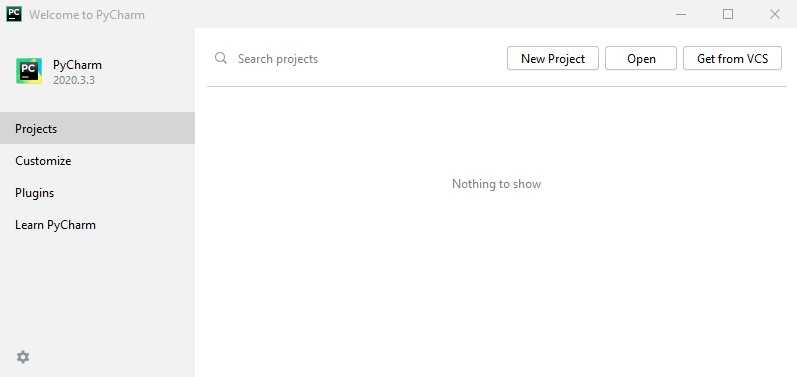
\includegraphics[width=0.65\textwidth]{pycharme.jpg}
	\end{center}
\end{block}
}	
\end{frame}

\section{Konfiguration}

\begin{frame}
\begin{block}{Settings importieren}
\vspace{2pt}
\begin{enumerate}
\item Lade Dir aus der Salem-Cloud die Datei \\ \texttt{Programmieren/Pycharm-Settings/pycharm\_settings.zip} \\ herunter und speichere sie auf Deinem Rechner.
\item Gehe in Pycharm auf \texttt{Customize > Import Settings...}
\item Wähle die zuvor heruntergeladene Datei aus. 
\item Führe einen Restart von Pycharm durch.
\item Falls Du einen Mac hast, stelle unter \texttt{Customize > Keymap} die Keymap \texttt{Salem-Mac} ein. 
\end{enumerate}
\end{block}
\end{frame}
	
\begin{frame}
\begin{block}{Interpreter einrichten}
\begin{enumerate}
\item Öffne Pycharm
\item Wähle \texttt{Project > New Project}
\item Dort kannst Du folgendes einstellen:
\begin{enumerate}
	\item Wähle unter \texttt{Location} einen Pfad, den Du auf Deinem Rechner wiederfindest
	\item Unter \texttt{Base Interpreter} wähle ein Python $\geq 3.6$ (Vorsicht: Der Punkt wird nicht immer mitgeschrieben)
	\item Setze einen Haken unter \texttt{Make available to all projects} 
	\item Setze den Haken unter \texttt{Create a main.py welcome script}
\end{enumerate}
\end{enumerate}	
\end{block}

\pause 

\begin{block}{So könnte es in etwa aussehen}
	
	\begin{center}
		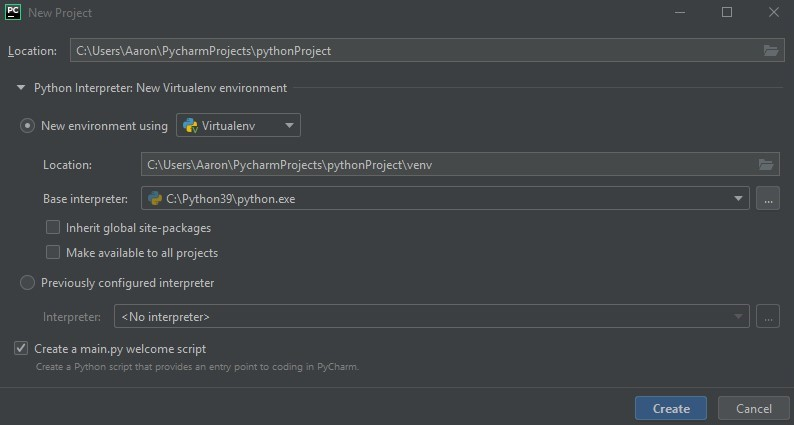
\includegraphics[width=0.5\textwidth]{python_interpreter.jpg}
	\end{center}
	
\end{block}

\end{frame}


\begin{frame}

\begin{block}{Nachdem Du auf \texttt{create} geklickst hast, sollte es etwa wie folgt aussehen}
\vspace{2pt}
	\begin{center}
		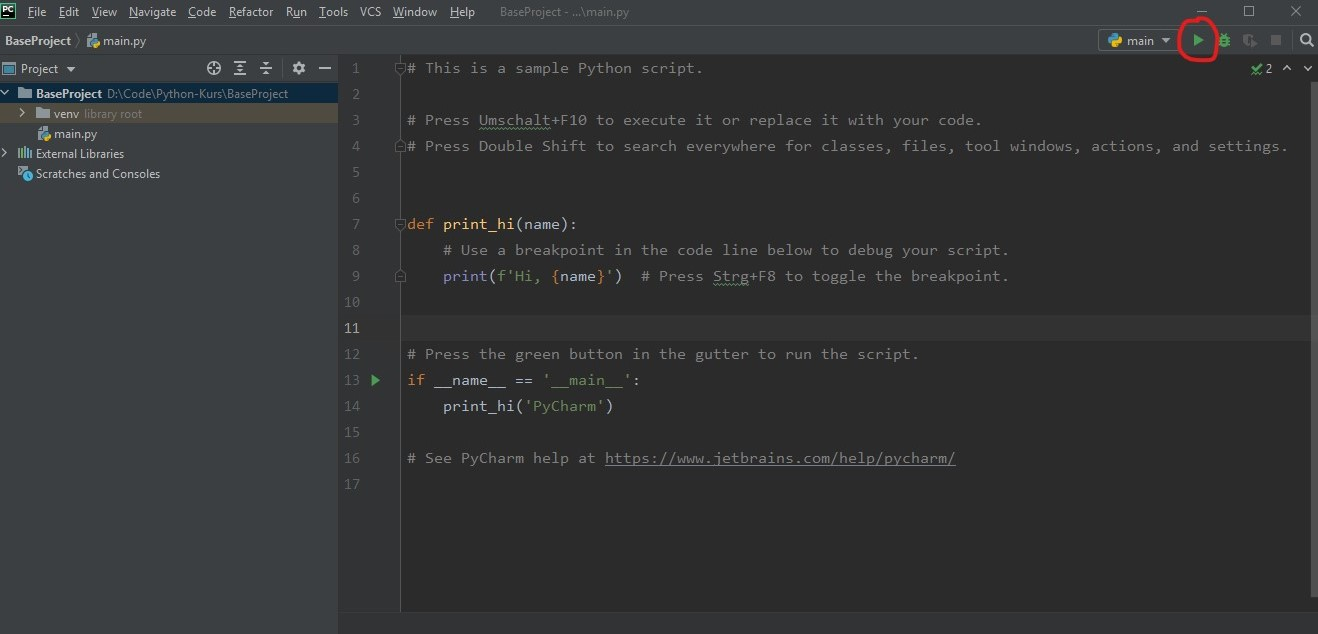
\includegraphics[width=0.85\textwidth]{pycharm_skript.jpg}
	\end{center}	



\end{block}

\end{frame}


\begin{frame}

\begin{block}{Den Code ausführen}
\vspace{2pt}
Klickst Du nun auf den grünen Pfeil oben rechts (siehe roter Kreis), sollte sich eine kleine Konsole öffnen und das Programm ablaufen. 
Alternativ kannst Du auch die Tastenkombination \texttt{Cmd + Enter} (Mac) bzw. \texttt{Strg + Enter} (Windows) verwenden.  

\pause

\begin{center}
	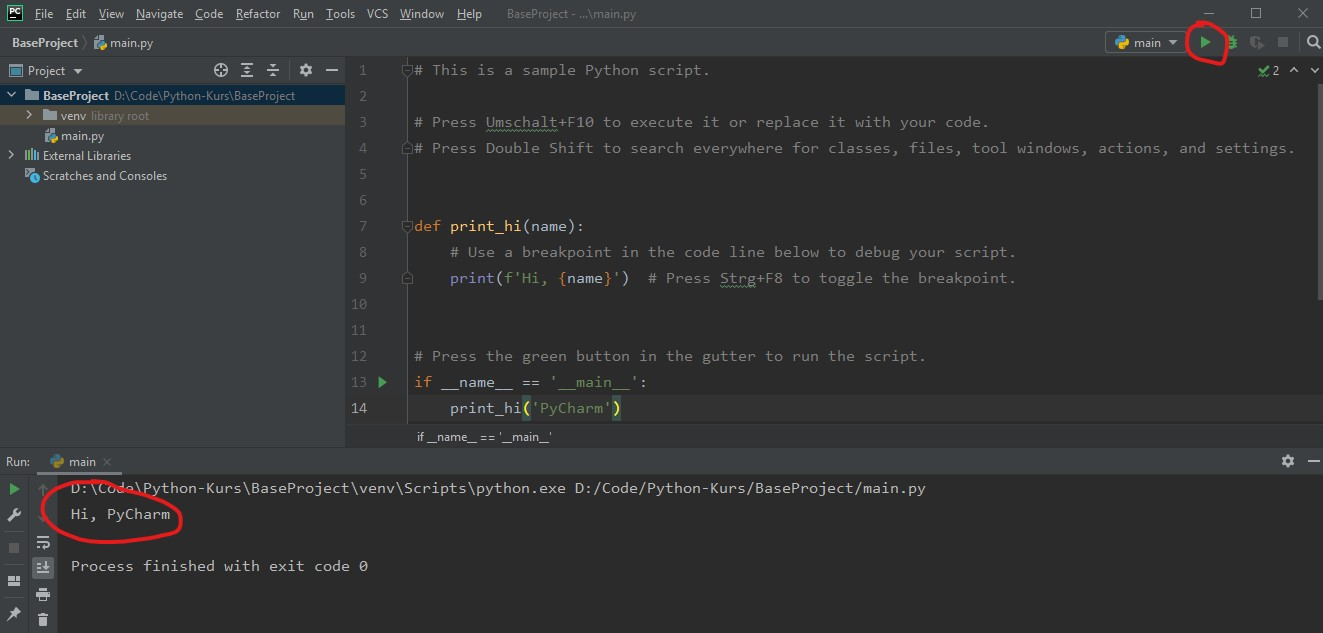
\includegraphics[width=0.85\textwidth]{pycharm_run.jpg}
\end{center}	

\end{block}

\end{frame}











\end{document}






